%\documentclass[a4paper,10pt]{article}
\documentclass[10pt, conference, letterpaper]{IEEEtran}
\usepackage[utf8]{inputenc}
\usepackage{xspace}
\usepackage{url}
\usepackage{graphicx,graphics} 
\usepackage{color}
\usepackage{amsmath}
\usepackage{amsfonts}
\usepackage{amssymb}
\usepackage{amsthm}
\usepackage{algorithm}
\usepackage{algorithmic}
\usepackage{longtable}
\usepackage{complexity}
\usepackage{tkz-graph}
\usepackage{float}
\usepackage{tabularx}
\usepackage{setspace}
\usepackage{icomma}
\renewcommand{\algorithmicrequire}{\textbf{Input:}}
\renewcommand{\algorithmicensure}{\textbf{Output:}}
\usepackage{authblk}
% \usepackage{hyperref}

\graphicspath{{figures/}}
\makeatletter
\def\input@path{{figures/}}
\makeatother
\newcommand\rmatching{${\cal R}$-matching\xspace}
\newcommand\mdelay{$\cal M$-delay\xspace}
\newcommand\matchedgraph{{\bf matched graph}}
\newtheorem{proposition}{Proposition}
\newtheorem{theorem}{Theorem}

\setlength{\parskip}{1ex} % Espace entre les paragraphes

\newtheorem{fact}{Fact}
\newtheorem{lemma}[theorem]{Lemma}
\newtheorem{definition}{Definition}
\newtheorem{corollary}{Corollary}

\renewcommand{\thefootnote}{\*}

\newcommand{\todo}[1]{{\color{red} TODO: {#1}}}
\newcommand\pazl{\textsc{pazl}\xspace}
\newcommand\pall{\textsc{pall}\xspace}
%opening
\title{Deterministic Scheduling of Periodic Messages for Cloud RAN}

\author{}

%\author[1]{Dominique Barth}
%\author[1]{Ma\"el Guiraud}
% \author[1]{Christian Cad\'er\'e}
%\author[2]{Brice Leclerc}
%\author[2]{Olivier Marc\'e}
%\author[1]{Yann Strozecki}
%\affil[1]{David Laboratory, UVSQ}
%\affil[2]{Nokia Bell Labs France}

\begin{document}

\maketitle

\begin{abstract}
A recent trend in mobile networks is to centralize in distant data-centers the processing units which were attached to 
antennas. The main challenge is to guarantee that the latency of the periodic messages sent from the antennas to their processing
units and back fulfills protocol time constraints. We show that traditional statistical multiplexing does not allow such a low latency, due to collisions and buffering at nodes. Hence, we propose in this article to use a deterministic scheme for sending periodic messages without collisions in the network thus without buffering and the resulting additional latency. 
We give several algorithms to compute such schemes for a common topology where one link is shared by all antennas.
We show that there is always a solution when the routes are short or the load is small. When the parameters are unconstrained,
and some buffering is allowed in the processing units, we propose an algorithm (PMLS) adapted from a classical scheduling method.
The experimental results show that even under full load, most of the time PMLS finds a deterministic sending scheme with no latency.
\end{abstract}

%\footnote{This work is partially supported by the french ANR project N-GREEN.}

%\section{Introduction}
%
%Next generations of mobile network architectures evolve toward centralized radio network architectures called C-RAN, or Cloud Radio Access Network, to reduce energy consumption costs~\cite{mobile2011c} and more generally the total cost ownership. The main challenge for this type of architecture is the latency in the periodic transfer process that is an important factor for dimensioning the network. The latency is measured between the sending of a message by the Remote Radio Heads (RRHs) on the field and the receptions of the answers, computed by real-time virtualized network functions on Baseband Units (BBUs), in the cloud. For example, even if next radio protocols are less stringent, some standards requires meeting time constraints for functions like HARQ (Hybrid Automatic Repeat reQuest) that needs to be processed in $3$ms~\cite{bouguen2012lte}. The specificity of the C-RAN context is not only the latency constraint, but also the periodicity of the data transfer in the \emph{frontaul} network between RRHs and BBUs.
%
%Let us expose briefly our model: the network topology is modeled by a directed weighted graph and a set of paths (routes) from source nodes (RRHs) to target nodes (BBUs). Time is discretized and a unit of time or slot corresponds to the transmission of a minimal unit of data over the network. The process must be  predictable (i.e. the date of arrival of packets is known beforehand). For simplicity, in this article we assume that the process is periodic. That is, if we look at the network at times $t$ and $t+P$ where $P$ is the period, all messages are at the same position in the network. Moreover, we want to avoid any  buffering in internal nodes of the graph. Hence we need to design a periodic process with no collision between messages. To ensure that this property is always true we propose a deterministic process.  We have two sets of values that we can choose when building a periodic sending process, called a \emph{periodic assignment} in this article: the time at which each packet is sent by a RRH in each period and the waiting time in the BBU before the answer is sent back to the RRH. When building a periodic assignment, we must take into account the periodicity which makes many scheduling methods inapplicable. Not only a message must not collide with the other messages sent by the others BBU/RRH in the same period, but also in the previous and following periods. Moreover the latency, that is the time between the emission of a message and the complete return of its answer, must be minimized. It means that the only buffering we are allowed -- the waiting time before sending back the answer-- must be small, in particular when the route is long. The aim is to operate a C-RAN on a low-cost shared switched network. The model is also compatible with an optical network with a fixed packet size.   


\section{Introduction}

Next generations of mobile network architectures evolve toward centralized radio network architectures called C-RAN, or Cloud Radio Access Network, to reduce energy consumption costs~\cite{mobile2011c} and more generally the total cost of ownership. The main challenge for this type of architecture is to reach a latency compatible with transport protocols. The latency is measured between the sending of a message by a Remote Radio Head (RRH) and the receptions of the answer, computed by real-time virtualized network functions of a BaseBand Unit (BBU) in the cloud. For example, LTE standards requires meeting time constraints for functions like HARQ (Hybrid Automatic Repeat reQuest) that needs to be processed in $3$ms~\cite{bouguen2012lte}. In 5G, some services need end to end latency as low as 1ms~\cite{3gpp5g}. The specificity of the C-RAN context is not only the latency constraint, but also the periodicity of the data transfer in the \emph{frontaul} network between RRHs and BBUs: frames need to be emitted and received every milliseconds~\cite{bouguen2012lte}.
Our aim is to operate a C-RAN on a low-cost shared switched network.
The question we address is the following: is it possible to schedule messages such that there is no collisions to avoid latency caused by queuing delays? 
Eliminating this source of latency leaves us with more time budget for latency coming from the length of the network, and thus allows for wider deployment areas.

Let us expose briefly our model: the network topology is modeled by a directed weighted graph and a set of paths (routes) from source nodes (RRHs) to target nodes (BBUs). Time is discretized and a unit of time or slot corresponds to the transmission of a minimal unit of data over the network. The process must be  predictable (i.e. the date of arrival of packets is known beforehand). Following LTE standard~\cite{bouguen2012lte}, in this article we assume that the process is periodic. That is, if we look at the network at times $t$ and $t+P$ where $P$ is the period, all messages are at the same position in the network. As we want to avoid any  buffering in internal nodes of the graph. Hence we need to design a periodic process with no collision between messages. To ensure that this property is always true we propose a deterministic process.  We have two sets of values that we can set when building a periodic sending process, called a \emph{periodic assignment} in this article: the time at which each packet is sent by a RRH in each period and the waiting time in the BBU before the answer is sent back to the RRH. When building a periodic assignment, we must take into account the periodicity which makes many scheduling methods unusable. Not only a message must not collide with the other messages sent by the others BBU/RRH in the same period, but also in the previous and following periods. The latency, that is the time between the emission of a message and the complete return of its answer must be minimized. This means that the only buffering we are allowed -- the waiting time before sending back the answer-- must be small, in particular when the route is long. Note that the model is technology agnostic, i.e. it is compatible with an optical network with a fixed packet size.   


%\footnote{Others terminologies and functional splits exist in the literature. We choose the most classical one for sake of clarity. The results of this work is fully compatible with any C-RAN architecture definition.}

Our main contributions are the following.
 In Sec.~\ref{sec:def} we propose a model of the network and the periodic sending of messages along its routes  and we introduce the star routed network that we study in this article. 
 We formalize the problem of finding a periodic assignment for sending messages without buffering (\pazl) or with buffering in the processing unit only (\pall) and shows that they are $\NP$-hard even to approximate. In Sec.~\ref{sec:PAZL}, we propose two algorithms solving \pazl when the routes between RRHs and BBUs are small or when the load is light. Using a compact representation of an assignment, we show that \pazl is fixed parameter tractable when parametrized by the number of antennas on star routed networks. Finally in Sec.~\ref{sec:PALL}, we introduce a family of algorithms to solve \pall and our experimentations allow to select one which works extremely well even in loaded networks. In particular we show that the deterministic communication schemes we design vastly outperform the traditional statistical multiplexing with regard to latency. 
 

   \subsection*{Related works}
   
 Statistical multiplexing even with a large bandwidth does not comply with the latency requirements of C-RAN. Therefore, the current solution~\cite{pizzinat2015things,tayq2017real} is to use dedicated circuits for the fronthaul. Each end-point, RRH or BBU, is connected through direct fiber or full optical switches. This architecture is very expensive and hardly scales in the case of a mobile network composed of tenths of thousands of deployment sites. The deterministic approach we propose has gained some traction recently: Deterministic Networking is under standardization in IEEE 802.1 TSN group~\cite{finn-detnet-architecture-08}, and in  IETF DetNet working group~\cite{ieee802}. Several patents on concepts and mechanisms for DetNet have been already published, see for example~\cite{howe2005time,leclerc2016transmission}. 
     
The algorithmic problem we focus on may look like wormhole problems~\cite{cole1996benefit}, but  we want to minimize the time lost in buffers and not just to avoid deadlocks. Several graph colorings have been introduced to model similar problems such as the allocation of frequencies~\cite{borndorfer1998frequency}, bandwidths~\cite{erlebach2001complexity} or routes~\cite{cole1996benefit} in a network or train schedules~\cite{strotmann2007railway}. Unfortunately, they do not take into account the periodicity of the scheduling and the associated problems are already $\NP$-complete. The only coloring with periodicity is the circular coloring~\cite{zhou2013multiple} but it is not expressive enough to capture our problem.

\section{Model and Problems}\label{sec:def}

  \subsection{Network modeling}
  

The network is modeled as a directed graph $G=(V,A)$. Each arc  $(u,v)$ in $A$ is labeled by an integer weight $\omega(u,v)$ which represents the time taken by a message to go from $u$ to $v$ using this arc. A {\bf route} $r$ in $G$ is a path, that is, a sequence of adjacent vertices $u_0, \ldots , u_{k}$, with $(u_i,u_{i+1}) \in A$.  The {\bf latency} of a vertex $u_i$ in a path $r$ is defined by $\lambda(u_i,r)= \sum\limits_{0 \leq j <i} \omega(u_j, u_{j+1})$.
% We also define $\lambda(u_0,r)=0$. 
The length of the route $r$ is defined by $\lambda (r)= \lambda (u_k,r)$.
We denote by $\cal R$ a set of routes, the pair $(G,\cal R)$ is called a {\bf routed network} and represents our telecommunication network. The first vertex of a route models an antenna (RRH) and the last one a data-center (BBU) which processes the messages sent by the antenna.

   In the context of cloud-RAN applications, we need to send message from a RRH $u$ to a BBU $v$ and then 
      we must send the answer from $v$ back to $u$. Therefore we assume that all considered routed networks 
      are \emph{symmetric}, that is for every arc $(u,v)$ there is an arc $(v,u)$ with the same weight.
      We define the function $\rho$ which associates to a route $r = u_0,\dots,u_k$ the symmetric route $\rho(r) = u_k,\dots,u_0$.
      The set ${\cal R}$ is partitioned into $F$ and $B$ such that $\rho$ is a bijection from $F$ to $B$.
      The routes of $F$ are called \textbf{forward} routes and those of $B$ are called \textbf{backward} routes.
%       
%       We say that a routed network $(G, {\cal R})$ is \textbf{symmetric} if the set of routes is partitioned into the sets $F$ of forward routes and $B$ of backward routes. Moreover there is a bijection $\rho$ between $F$ and $B$ such that for any forward route $r \in F$ with first vertex $u$ and last vertex $v$, the backward route $\rho(r) \in B$ has first vertex $v$ and last vertex $u$.
%       In all practical cases the routes $r$ and $\rho(r)$ will be the same with the orientation of the arcs reversed, which corresponds to bidirectional links in the networks, but we need not to enforce this property.
      


   \subsection{Messages dynamic}
      
      
      In the process we study, a message is sent on each route at each period, denoted by $P$.
      Let $r$ be a route, if a message is sent at time $m$ from $s$ the first vertex of $r$ then it will arrive at vertex $v$ in $r$ at time $m + \lambda(v,r)$. Since the process is periodic, if we look at the messages going through an arc between time $0$ and $P-1$, then we see the same messages in the same order and position between time $kP$ and $(k+1)P -1$ for all $k$. 
      Therefore, the first time slot at which a message sent at time $m$ on $r$ reaches a vertex $v$ in $r$ is $t(v,r) = m + \lambda(v,r) \mod P$. 
      
      A message usually cannot be transported in a single time slot. We denote by $\tau$ the number 
      of \emph{consecutive slots} necessary to transmit a message. Let us call $[t(v,r)]_{P,\tau}$ the set of time slots used by route $r$ at vertex $v$ in a period $P$, that is $[t(v,r)]_{P,\tau} = \{t(v,r) + k \mod P \mid 0 \leq k < \tau \}$. Usually $P$ and $\tau$ will be clear from the context and we will denote $[t(v,r)]_{P,\tau}$ by $[t(v,r)]$.
      Let $r_1$ and $r_2$ be two routes, on which messages are sent at time $m_1$ and $m_2$ in their first vertex.
      We say that the two routes have a {\bf collision} if they share an arc of first vertex $v$ and $[t(v,r_{1})] \cap [t(v,r_{2})] \neq \emptyset$.
      
         A {\bf $(P,\tau)$-periodic assignment} of a routed network $(G,\cal R)$ is a function that associates to each route 
         $r \in \cal R$ its \textbf{offset} $m_r$ that is the time at which a message is emitted at the first vertex of the route $r$. \emph{No pair of routes must have a collision} in a $(P,\tau)$-periodic assignment.
	 An assignment represents the following process: first a message is sent at $u$, through the forward route $r$, at time $m_r$.
      \begin{center}
     \hspace{-0.5cm} 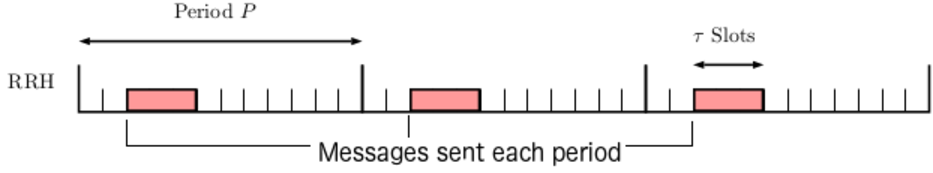
\includegraphics[width=0.48\textwidth]{rrh.pdf}
      \end{center}

      This message is received by $v$ the last vertex of $r$ at time $t(v,r)$. It is then sent back to $u$ on the route $\rho(r)$ in the same period at time $m_{\rho(r)}$ if $m_{\rho(r)} > t(v,r)$, otherwise at time $m_{\rho(r)}$ in the next period. The time between the arrival of the message and the time it is sent back is called the \textbf{waiting time} and is defined by $w_r = m_{\rho(r)} - t(v,r)$ if $m_{\rho(r)} > t(v,r)$ and $w_r = m_{\rho(r)} + P - t(v,r)$ otherwise.
 
       \begin{center}
     \hspace{-0.5cm} 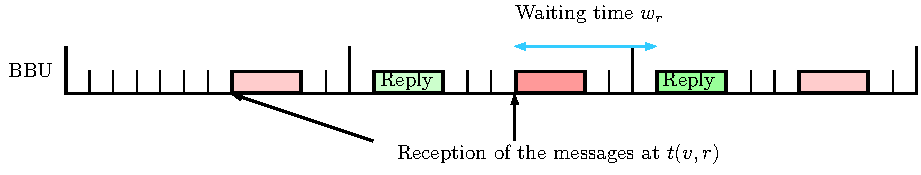
\includegraphics[width=0.48\textwidth]{BBU.pdf}
      \end{center}
     
    
      Thus, the whole process time for a message sent on the route $r$ is equal to
      $PT(r)=\lambda(r)+ w_r+\lambda(r)$.      
      In the process time, we count the time between the first time at which a message is emitted and the first time at which the message comes back. 
%       Alternatively we could consider the time between the emission of the first slot and the reception of the last slot of the message, which would add $\tau$ to the process time.
%       However, since all messages are of size $\tau$, it will not change the problems we consider in the rest of the article.
      Finally, we should add to the process time the computation time that a BBU needs to deal with one message, but it can be encoded  in the weight of the last arc leading to the BBU and thus we need not to consider it explicitly in our model.

    
      \subsection{Periodic assignment for low latency}
      
      
    The {\bf maximum process time} of the assignment $m$ of $(G,{\cal R})$ is defined by $MPT(m)=\max\limits_{r \in {\cal R}} PT(r)$. We consider the following decision problem.

      \noindent {\bf Periodic Assignment for Low Latency (\pall)} 

      \noindent {\bf Input:}  A routed network $(G,{\cal R})$, the integers $P$, $\tau$ and $T_{max}$.

      \noindent {\bf Question:} does there exist a $(P,\tau)$-periodic assignment $m$ of $(G,{\cal R})$ such that $MPT(m) \leq T_{max}$?

%       In Sec.~\ref{sec:\pall} we will study algorithms which solve the search version of \pall (computing an assignment), also denoted by \pall for simplicity. \todo{phrase utile finalement ?} 
      It turns out that the problem \pall is hard to solve for \emph{general} routed networks. The long version of this article contains complete proofs of the $\NP$-hardness or hardness of approximation of \pall and of several of its variants.

 \begin{theorem}
Problem \pall is $\NP$-complete.
\end{theorem}

\noindent \emph{Sketch of proof:}
 First, by a symmetry argument, the problem of finding an assignment with no collisions for the forward routes only
 can be reduced to \pall.
 We fix $\tau$ the size of messages to $1$ and we reduce the problem of $k$-coloring to the 
 problem of finding an assignment without collisions for the forward routes.
 Let $H$ be a graph instance of the $k$-coloring problem, from it we build a routed network $(G,{\cal R})$. 
 For each vertex $v$ in $H$, there is a route $r_v$ in ${\cal R}$. Two routes $r_v$ and $r_u$ share an arc if and only if $(u,v)$ is an arc in $H$; this arc is the only one shared by these two routes. All arcs are of weight $0$. 
 Observe that the existence of a $k$-coloring of $H$ is equivalent to the existence of a $(k,1)$-periodic assignment in $G$, 
 by converting an offset of a route into a color of a vertex and reciprocally. \qed
     
       We also consider a simpler version of \pall, that we call {\bf Periodic Assignment for Zero Latency} or \pazl: we ask for a $(P,\tau)$-periodic assignment {\bf with all waiting times equal to $0$}. We introduce \pazl because it is simpler to study and we are able to prove theoretical results and find better algorithms than for \pall. As we  experimentally show in Sec.~\ref{sec:exp_PAZL}, this problem can often be solved positively albeit less often than the general problem. Finally, a solution to \pazl is simpler to implement in real telecommunication networks, since we do not need any buffering at all.    
       
 
 
    \subsection{The star routed network}
    
      Let us define a family of simple routed networks modeling a Point-to-Multipoint fronthaul (PtMP), which has been designed for C-RAN \cite{tayq2017real}. 
      The graph $G$ has two sets of vertices, $S=\{s_0,...,s_{n-1}\}$ and $T=\{t_0,...,t_{n-1}\}$ of cardinality $n$ and two special nodes, the central source node $c_s$ and the central target node $c_t$.
      There is an arc between $c_s$ and  $c_t$ called the central arc and for all $i<n$ there is an arc between $s_i$ and $c_s$ and between $t_i$ and $c_t$. All the symmetric arcs are also in the graph with the same weights.
      The forward routes are the directed paths $r_i = (s_i,c_s,c_t,t_i)$ and the backward routes are $\rho(r_i) =(t_i,c_t,c_s,s_i)$. The routed network $(G, \{r_i,\rho(r_i)\}_{i<n})$ is called a \textbf{star routed network}. 
       
       \begin{center}
	 \scalebox{0.6}{
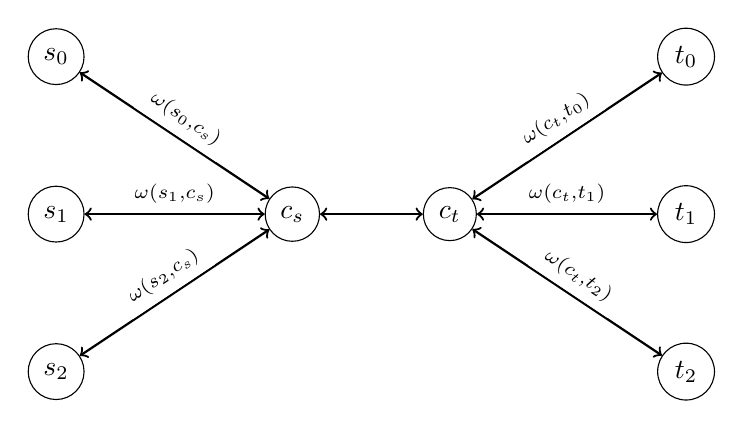
\begin{tikzpicture}

\tikzset{EdgeStyle/.style={<->,font=\scriptsize,above,sloped,midway}}
  \SetGraphUnit{5}
  
  \node[draw,circle] (s3) at (0, 0) {$s_2$}; 
  \node[draw,circle] (s2) at (0, 2) {$s_1$}; 
  \node[draw,circle] (s1) at (0, 4) {$s_0$}; 

  \node[draw,circle] (t3) at (8, 0) {$t_2$}; 
  \node[draw,circle] (t2) at (8, 2) {$t_1$}; 
  \node[draw,circle] (t1) at (8, 4) {$t_0$}; 
  

  \node[draw,circle] (cs) at (3, 2) {$c_s$}; 
  \node[draw,circle] (ct) at (5, 2) {$c_t$}; 

  
  \Edge[label = $\omega({s_0,c_s})$](s1)(cs)
  \Edge[label = $\omega({s_1,c_s})$](s2)(cs)
  \Edge[label = $\omega({s_2,c_s})$](s3)(cs)
  
  \Edge[label = $\omega({c_t,t_0})$](ct)(t1)
  \Edge[label = $\omega({c_t,t_1})$](ct)(t2)
  \Edge[label = $\omega({c_t,t_2})$](ct)(t3)
  
  \Edge(cs)(ct)

  
\end{tikzpicture}
}

  \end{center}
  
  Since the central arc appears in every route, its value does not matter when considering the process time of an assignment.
  Moreover an assignment without collisions is also an assignment without collisions of the same star routed network with the weight of the central arc set to $0$. Hence, we assume from now on that the weight of the central arc is $0$.
      
      
  Collisions between messages can only appear on the arc $(c_s,c_t)$ between forward routes or on the arc $(c_t,c_s)$
  between backward routes. The flow of messages in a star routed network is completely described by their repartition in two time windows of size $P$ that we call the {\bf forward period} (at $(c_s,c_t)$), and the {\bf backward period} (at $(c_t,c_s)$).

  Star routed networks seem really simple, but \pall or \pazl may be $\NP$-hard restricted to these networks.
  We conjecture it is the case since  a variant of \pazl where the central link is unidirectional (collisions can happen between forward and backward routes) can be shown to be $\NP$-complete. It is done by a reduction from the subset sum problem as for a similar problem of scheduling pair of tasks~\cite{orman1997complexity}. 
      
%
%      
%      A {\bf $(P,\tau)$-periodic assignment} of a routed network $(G,\cal R)$ is a sequence  $m=(m_0, \ldots ,m_{n-1})$ of $n$ integers that we call {\bf offsets}, with $n$ the number of routes in $\cal R$. The number $m_{i}$ represents the time at which a message is emitted at the first vertex of the route $r_{i}$. We will always consider that the $m_{i}$ are between $0$ and $P-1$. Moreover, \emph{no pair of routes must have a collision} in a $(P,\tau)$-periodic assignment.
%
%      As an example of a $(2,1)$-periodic assignment, let us consider a routed network 
%      where all pairs of routes intersect at a different arc. It is easy to design such a network and an example is given in Fig.~\ref{fig:example}. We set $\tau = 1$ and the weights are chosen so that if $r_{i}$ and $r_{j}$ have $v$ as first common vertex then we have $\lambda(v,r_{i}) - \lambda(v,r_{j})=1$. There is a $(2,1)$-periodic assignment by setting all $m_{i}$ to $0$.
%
%  
%      \begin{figure}[ht]
%      \begin{center}
%          \scalebox{0.5}{
%          
%\begin{tikzpicture}
%
%
%\tikzset{
%  LabelStyle/.style = { rectangle, rounded corners, draw,
%                       font = \bfseries },
%  EdgeStyle/.append style = {->} }
%  \SetGraphUnit{5}
%  \node[draw,circle] (s3) at (4, 2) {$s_2$}; 
%  \node[draw,circle] (s2) at (0, 4) {$s_1$}; 
%  \node[draw,circle] (s1) at (0, 6) {$s_0$}; 
%
%  \node[draw,circle] (t3) at (14, 7) {$t_2$}; 
%  \node[draw,circle] (t2) at (14, 4) {$t_1$}; 
%  \node[draw,circle] (t1) at (10, 2) {$t_0$}; 
%
%  
%  \SetVertexNoLabel
%  \Vertex[x=2,y=5]{A}
%  \Vertex[x=4,y=5]{B}
%  \Vertex[x=10,y=5]{C}
%  \Vertex[x=12,y=5]{D}
%  \Vertex[x=6,y=3]{E}
%  \Vertex[x=8,y=3]{F}
%  \tikzset{
%  EdgeStyle/.append style = {green} }
%  \Edge[label = 2](s2)(A)
%  \Edge[label = 1](A)(B)
%  \Edge[label = 2](B)(C)
%  \Edge[label = 1](C)(D)
%  \Edge[label = 1](D)(t2)
%
%  
%   \tikzset{
%  EdgeStyle/.append style = {red} }
%  \Edge[label = 2](s3)(E)
%  \Edge[label = 1](E)(F)
%  \Edge[label = 1](F)(C)
%  \Edge[label = 1](C)(D)
%  \Edge[label = 1](D)(t3) 
%     \tikzset{
%  EdgeStyle/.append style = {blue} }
%  \Edge[label = 1](s1)(A)
%  \Edge[label = 1](A)(B)
%  \Edge[label = 1](B)(E)
%  \Edge[label = 1](E)(F)
%  \Edge[label = 1](F)(t1)
%
%\end{tikzpicture}
%
%}
%     \end{center}
%       \caption{A routed network with $(0,0,0)$ as a $(2,1)$-periodic assignment}
%       \label{fig:example}
%      \end{figure}
%
%      \subsection{Periodic route assignment}\label{nonmonotone}
%
%    We want to find an assignment which allows to send periodic messages from sources to targets
%    without collisions. We introduce the following associated decision problem, useful for hardness proofs.
%    
%
%      \noindent {\bf  Periodic Routes Assignment (PRA)} 
%
%      \noindent {\bf Input:} a routed network $(G,\cal R)$, an integer $\tau$ and an integer $P$.
%
%      \noindent {\bf Question:} does there exist a $(P,\tau)$-periodic assignment of $(G,\cal R)$ ?
%
%
%      We will prove in Sec.~\ref{sec:complexity} that the problem PRA is $\NP$-complete, even in restricted settings.
%      In fact, approximating the smallest value of $P$ for which there is a $(P,\tau)$-periodic assignment is already hard.
%        
%   An unusual property of assignment is that given a routed network, we may have a $(P,\tau)$-periodic assignment but no
%	\begin{lemma} \label{lemma:monotonic}
%	 For any odd $P$, there is a routed network such that there is $(2,1)$-periodic assignment but no $(P,1)$-periodic assignment.
%	\end{lemma}
%\begin{proof}
%
%      Consider the routed network $(G,{\cal R})$ given in the previous subsection. 
%      We change the weights so that for $v$, the first vertex which belongs to $r_i$ and $r_j$,
%      we have $\lambda(v,r_i) - \lambda(v,r_j)= P$, where $P$ is an odd number smaller than $n$, the number of routes in ${\cal R_{\cal C}}$. In such a graph, there is no $(P,\tau)$-periodic assignment, since the problem reduces to finding a $P$-coloring in a complete graph with $n > P$ vertices, the colors being the offsets of the routes.\\
%      If we consider a period of $2$, for all $i \neq j$, $\lambda(v,r_i) - \lambda(v,r_j) \mod 2 = 1$ . Therefore $(0,\dots,0)$ is a $(2,1)$-periodic assignment of ${\cal R}$.      
%\end{proof}
      
      
         \section{Solving \pazl on Star Routed Networks}\label{sec:PAZL}
         
       In this section, we deal with the problem PAZL on star routed networks. Since we want an assignment with waiting times zero, $MPT(m)$ is equal to twice the length of the longest route, thus $T_{max}$ is not relevant anymore. Moreover choosing the offset $m_r$ of a forward route $r$ also sets the offset of the backward route $\rho(r)$ to $m_{\rho(r)} = m_{r} + \lambda(r) \mod P$.  Consider an assignment $m$ of a star routed network and let $m'_r= m_{r} - t(c_s,r) \mod P$. Then $m'$ is an assignment of the same star routed network where, for all $i$, the weights of the arcs $(s_i,c_s)$ are set to $0$. Therefore we assume from now on that the \emph{weight of the arcs $(s_i,c_s)$ are all equal to $0$}.
      
      
\subsection{Shortest-longest policy}
    

    We first present a simple policy, which works when the period is large with regard to the lengths of the routes.
    The messages are sent in order from the shortest route to the longest route, without any gap between two messages in the forward period.
    In other words, we assume that the route $r_i$ are sorted by increasing $\lambda(r_i)$ and we set $m_{r_i}$ the offset of $r_i$ to $i\tau$. We call this algorithm {\bf Shortest-Longest}.
      
     By definition, there are no collision in the forward period and if the period is long enough, 
     it is easy to see that in the backward period the order of the messages are the same as in the forward period and that no collision can occur. 
      
      
      \begin{proposition} Let $(G, {\cal R})$ be a star routed network, and let $n\tau + 2(\lambda(r_{n-1}) - \lambda(r_{0})) \leq P$. There is a $(P,\tau)$-periodic assignment of $(G, {\cal R})$ with waiting times $0$ given by Shortest-Longest.\label{prop:SL}
      \end{proposition}
      \begin{proof}
       Since $m_{r_i} = i\tau$, $[t(c_s,r_{i})] = \{i\tau,\dots, (i+1)\tau -1\}$ and there are no collision on the forward period.
       
       
       We may assume that $\lambda(r_{0}) = 0$, since removing $\lambda(r_{0})$ from every arc $(c_t,t_i)$ does not change the order on the length of the routes nor the collisions between messages.
       Since $\lambda(r_{0}) = 0$, by hypothesis we have $n\tau + 2\lambda(r_{n}) \leq P$ which implies that
       $[t(c_t,r_{i})] = \{2 \lambda(r_{i}) + i\tau, \dots,  2 \lambda(r_{i}) + (i+1)\tau -1\}$.
       Since $ \lambda(r_{i}) \leq  \lambda(r_{i+1})$ by construction, we have  $2 \lambda(r_{i}) + i\tau -1 < 2 \lambda(r_{i+1}) + (i+1)\tau$ which proves that there are no collision on the backward period. 
%        The complexity of the algorithm is dominated by the sorting of the routes in $O(n\log(n))$. 
      \end{proof}

      If the period is slightly smaller that the bound of Proposition~\ref{prop:SL}, a collision will occur on the first route in the backward period. Hence, this policy is not useful even as a heuristic for longer routes as confirmed by the experimental results of Subsection~\ref{sec:exp_PAZL}. 

   
    \subsection{Greedy algorithm}
    
    
      We define the \textbf{load} of a star routed network as $\frac{n\tau}{P}$, it is the proportion of time slots used by messages on the central arc in a period. Therefore if the load is larger than $1$ there cannot be an assignment. We propose a greedy algorithm to build a $(P,\tau)$-periodic assignment, which always finds an assignment when the load is less than $1/3$. Therefore in the rest of the article we will be only concerned with load larger than $1/3$.
    
    \begin{proposition}
    There is a $(P,\tau)$-periodic assignment of a star routed network with waiting times $0$ if the load is less than $1/3$.
%     and it can be found in time $O(n^2)$.
    \end{proposition}
    \begin{proof}
     We consider the forward period and cut it into consecutive intervals of size $\tau$ that we call macro-slots. The algorithm works by choosing an offset for each route in the following way: try all offsets which put the message in a yet not used macro-slot in the forward
     period. Since the choice of an offset also fixes the position of the message in the backward period, chose the first one which does not create a collision. We now prove that this algorithm always finds a $(P,\tau)$-periodic assignment without waiting time when $P \geq 3n\tau$ that is the load is less than $1/3$.
     
     Assume we are choosing the offset of the route $r_{k+1}$, we have at least $P - k \geq 3n - k$ free macro-slots in the forward period, since $P \geq 3n\tau$. Each of these $3n - k$ possible offset values translates into $3n - k$ positions of messages in the backward period. All these positions are separated by at least $\tau$ slots. There are already $k$ messages of size $\tau$ in the backward period. One such message can intersect at most $2$ potential positions since they are disjoint intervals. Therefore  amongst the possible $3n - k$ positions, there are  at least $3n - k -2k$ which are without collision. Since $k < n$, $3n - k -2k \geq 1$, which proves that the algorithm terminates and find a  $(P,\tau)$-periodic assignment. 
%      
%      This algorithm works with a complexity $O(n^2)$, since for the $k^{\text{th}}$ route we have to try at most $2k$ offsets before finding a correct one. We can test the $2k$ offsets of the backward period in time $O(k)$ by maintaining an ordered list of the intervals used by already set routes.
     \end{proof}
     
      \begin{center}
      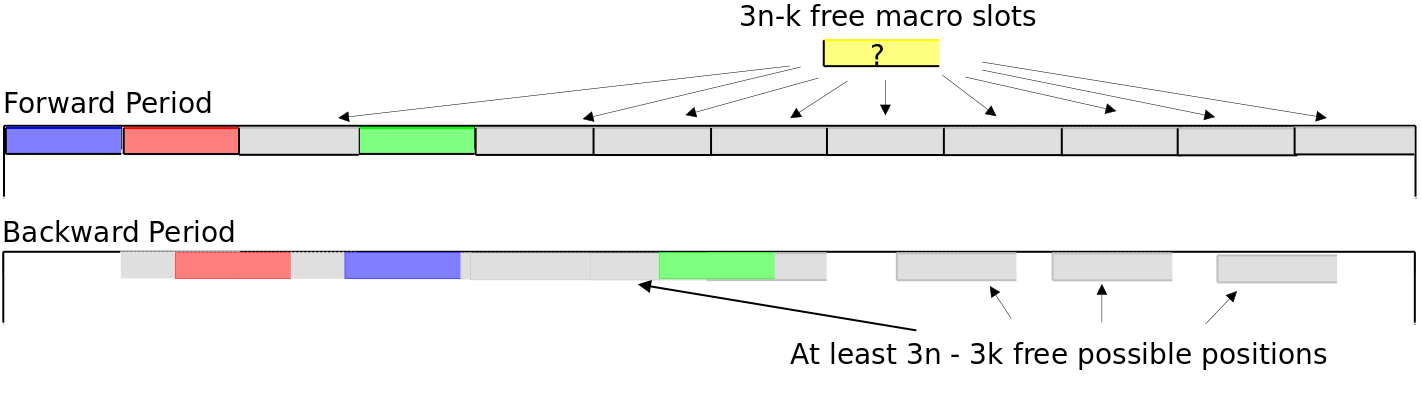
\includegraphics[width=0.48\textwidth]{ex3nt.png}
      \end{center}
% 	\begin{algorithm}[H]
% 	\caption{Greedy assignment}
% 	\begin{algorithmic}
% 	\REQUIRE ${\cal R}_{\cal C}$, period $P$
% 	\ENSURE A P-periodic assignment in p $\leq P$, or FAILURE
% 	\STATE $T$ a table of the macro slots of size $\tau$ in the forward period.
% 	\STATE $L$ a list of free intervals in the backward period%$P2[P]$ slots backward period.
% 	\FORALL{source $s$ in S}
% 
% 	\FORALL{free intervals $[a,b]$ in $L$}
% 	\FORALL{ $a/\tau - \lambda(s) <j< b/\tau - \lambda(s)$ }
% 	\IF{ $T[j] == FREE$}
% 	\STATE $m_{s} \leftarrow j.\tau$
% 	\STATE $T[j] = USED$
% 	\STATE update $[a,b]$ in $L$
% 	\STATE BREAK
% 	\ENDIF
% 	\ENDFOR
% 	\ENDFOR
% % 	
% % 	\IF{No intervals are found for $s_i$}
% % 	\STATE return FAILURE
% % 	\ENDIF
% % 	\ENDFOR
% 
% 	\ENDFOR
% 
% 	\end{algorithmic}
% 	\end{algorithm}
	
This algorithm, contrarily to the previous one, may work well, even when the condition on the load is not true.
In fact, experimental data in Subsection~\ref{sec:exp_PAZL} suggests that the algorithm finds a solution when the load is less than $1/2$. Note that we have experimented with other greedy algorithms which do not use macro-slots, they work even better in practice but their theoretical upper bound is worse.

\subsection{An FPT algorithm}

In this section we show how every assignment without waiting time can be put into a canonical form.
We use that to provide an algorithm which finds an assignment when it exists, in fixed parameter tractable time ($\FPT$) with parameter $n$ the number of routes (for more on parametrized complexity see~\cite{downey2012parameterized}). This is justified since $n$ is small in practice and the other parameters such as $P$, $\tau$ or the weights are large.

Let $(G, {\cal R})$ be a star routed network and $m$ a $(P,\tau)$-periodic assignment.
A set of routes $S$ is \textbf{coherent} if for all $r \in {\cal R}$, $r \in S$ if and only if $\rho(r) \in S$. We say that a coherent set $S \subseteq {\cal R}$ is \textbf{compact} for the assignment $m$ if there is a route $r_0 \in S$ such that the following holds:  
for all coherent subsets $S'\subset S$ with $r_0 \notin S'$, if we remove $1$ from all offsets of routes in $S'$ then there is a collision with a route of $S \setminus S'$. We say that $m$ is compact if ${\cal R}$ is compact for $m$. 
% 
% 
% $r_1,r_2 \in {\cal R}$ two forward routes (resp. two backward routes) and 
%  We say that there is no gap between $r_1$ and $r_2$ in $\mathcal{M}$ if $\lambda(r_1,c_s) + \tau = \lambda(r_2,c_s)$ (resp. $\lambda(r_1,c_t) + \tau = \lambda(r_2,c_t)$). It means that the message of $r_2$ goes through the central arc just after the message of $r_1$ withtout wasting time. We say that a set of routes ${\cal R}$ is \textbf{compact} for the assignment $\mathcal{M}$ if for all forward routes $r \in {\cal R}$ but one, there is another forward route $r'$ such that there is no gap between $r'$ and $r$ or between $\rho(r')$ and  $\rho(r)$. If the set of all routes is compact for an assignment, we say that the assignment is compact.

\begin{proposition}
Let $(G, {\cal R})$ be a star routed network. If there is a $(P,\tau)$-periodic assignment of $(G, {\cal R})$, then there is a compact $(P,\tau)$-periodic assignment of $(G, {\cal R})$.
\end{proposition}
\begin{proof}
Consider $m$ a $(P,\tau)$-periodic assignment of $(G, {\cal R})$.
Let $r_0$ be an arbitrary route of ${\cal R}$,  and let $COMP = \{r_0\}$. Now we apply the following algorithm to $m$ and $COMP$ while $COMP$ is not equal to ${\cal R}$.
While there is no collision, remove $1$ (modulo $P$) from all offsets of routes in ${\cal R} \setminus COMP$. Then choose a route $r$ in ${\cal R} \setminus COMP$ which would have a collision with a route $r'$ of $COMP$ if one is subtracted from its offset. If $r'$ is a forward route, let $COMP = COMP \cup \{r, \rho(r)\}$ otherwise  $COMP = COMP \cup \{r, \rho^{-1}(r)\}$. 

We prove by induction that $COMP$ is compact for $m$ at every step of the algorithm.
At the beginning $|COMP| = 1$ and the property is trivially satisfied. Then we assume that 
$COMP$ is compact and that we add to it $\{r, \rho(r)\}$ at some step of the algorithm. W.l.o.g we assume that it is the offset of $r$ which cannot be decremented without collision. Consider $S \subseteq   COMP$, if $S$ contains an element different from $r$ and $\rho(r)$ by induction hypothesis we cannot decrement the offsets of $S$ without collision. If $S =\{r, \rho(r)\}$
by construction, we cannot decrement the offset of $r$. 

Finally, there is no collisions between routes at the beginning and since we modify $m$ only if it creates no collision, the assignment we obtain at the end has no collisions between routes.
\end{proof}

We now present an algorithm to find a $(P,\tau)$-periodic assignment 
by trying all compact assignments.

\begin{theorem}\label{th:FPT}
$\pall \in \FPT$ when parametrized by the number of routes.
\end{theorem}
\begin{proof}
Let $(G, {\cal R})$ be a star routed network and let $m$ be a $(P,\tau)$-periodic assignment of $(G, {\cal R})$. First remark that for a given assignment and a route $r_0$ with offset $m$, by removing $m$ to all offsets, we can always assume that its offset is zero. Therefore we need only to consider all \emph{compact assignments} with an \emph{offset $0$} for the route $r_0$. 
We now evaluate the number of compact assignments and prove that it only depends
on $n$ the number of routes which proves the theorem. 
We give a way to build a compact assignment $m$ by determining its offsets one after the other. We fix an arbitrary total order on ${\cal R}$.
First a route $r_0$ is chosen arbitrarily and its offset set to $0$. 
Then at each step, if the offsets of $S \subseteq  {\cal R}$ have been chosen,
we select the smallest route $r$ in $S$ for the order. 
Then we select a route in $r' \in {\cal R} \setminus S$ and set its offset such that 
if we remove $1$ then $r'$ collides with $r$. Note that if $r$ is a forward route (resp. a backward route) then $r'$ is also a forward route (resp. a backward route). We can also decide to definitly skip $r$. At a given step of the algorithm, if $|S| = 2i$, we have $n-i$ choices 
of routes to select. The value of the offset of the selected route is entirely determined by the values of the offsets of routes in $S$. Therefore there are at most $n!$ different compact assignments with offset $r_0$ fixed to $0$. 

The algorithm to solve \pall builds every possible compact assignment as described here, and
tests at each step whether there is a collision which can be done in time linear in the size of 
$(G, {\cal R})$. Therefore $\pall \in \FPT$.
\end{proof}

We call the algorithm described in Theorem~\ref{th:FPT} \textbf{Exhaustive Search of Compact Assignments}. To make it more efficient in practice, we make cuts in the search tree used to explore all compact assignments. Consider a set of $k$ forward routes whose offsets has been fixed at some point in the search tree. We consider the times at which the messages of these routes cross the central arc. It divides the period into $[(a_0,b_0), \dots, (a_{k-1},b_{k-1})]$ such that the central arc is free only during the intervals $(a_i,b_i)$. Therefore at most $\displaystyle{ \sum_{i=0}^{k-1} \lfloor(b_{i} -a_i)/\tau\rfloor} $ forward routes can still use the central arc. If this value is less than $n - k$, it is not possible to create a compact assignment by extending the one on $S$ and we backtrack in the search tree. The same cut is used for the backward routes.
% 	\subsubsection*{Exhaustive search}
% % 	\begin{algorithm}[H]
% % 	\caption{Exhaustive Generation}  
% % 	\begin{algorithmic}
% % 	\REQUIRE A routage graph ${\cal R}_{\cal C}$, period $P$, packet size $\tau$
% % 	\ENSURE $(P,\tau)$-periodic assignment of ${\cal R}_{\cal C}$
% % 	\STATE Forward-budget $\leftarrow$ $P$ - n * $\tau$
% % 	\STATE Backward-budget $\leftarrow$ $P$ - n * $\tau$
% % 	\STATE Free-Intervals $\leftarrow$ list of free intervals in the backward period, init to $[0;P[$
% % 	\FORALL{source $s_i$ in S}
% % 	\FORALL{j in Free-Intervals }
% % 	\IF{Message of the route $r_{s_i}$ does not collides with scheduled routes}
% % 	\STATE $m_{s_i} \leftarrow $ the first slot of Free-Intervals[j]
% % 	\STATE Split the Free-Intervals considering the new packet
% % 	\STATE Forward-budget $\leftarrow$ Forward-budget - {\em lost size}
% % 	\STATE Backward-budget $\leftarrow$ Backward-budget - {\em lost size}
% % 	\STATE call Exhaustive Generation on remaining routes
% % 	\ENDIF
% % 	\ENDFOR
% % 	\ENDFOR
% % 
% % 
% %       \end{algorithmic}
% %       \end{algorithm}
% 
% % 	    
%       We now present an exhaustive search algorithm, which tries to set the offsets in all possible ways until it has found a $(P,\tau)$-periodic assignment. Contrarily to the two previous algorithms, when it fails to find a solution, then it certifies there are no solution to PAZL.
%       
%       We have $n$ routes denoted by $\{0,\dots,n-1\}$. A partial solution $S$ is 
%       a partial function from $[n]$ to $\{0,1,\dots,P-\tau -1\}$ which sets a starting time for a subset of the routes $R(S) \subseteq [n]$, such that there are no collisions for these routes.  A partial solution $S'$ extends $S$, if $S'$ is defined over one more route than $S$ and this route has a larger starting offset than all routes of $S$: $R(S') = R(S) \cup \{r'\}$ and for all  $r \in R(S)$, $S(r) + \tau \leq S'(r')$. We define a tree whose nodes are partial solutions and such that the root is the empty partial solution and the children of a partial solution are the partial solutions which extend it. The solutions to our problem will be the leaves of depth $n$ in the tree, and our exhaustive search algorithm is a depth-first search of this tree. 
%       
%       Remark that a node $S$ with $|R(S)| = k$ can have as many as $(n-k)P$ children. Since the tree is of depth $n$, the tree may have as many as $n!P^n$ elements and while $n$ is small, $P$ may be large which makes its traversal intractable.  Therefore we have to find cuts in the tree to avoid to explore it entirely and henceforth make the algorithm practical. Cuts correspond to the detection of subtrees which contain no solutions or solutions which can be found elsewhere and can thus be skipped. We now propose three cuts, the first two being particularly useful when the network is loaded ($n\tau$ is not far from $P$). 
%       
%       \begin{enumerate}
%        \item We consider the number of slots which can be used by routes not yet fixed by a partial solution in the \emph{forward period}. When we extend a solution into $S$ with a new route at offset $m$, then at most $(P - m) / \tau $ routes can still be used to extend $S$ without collisions in the forward period. If that value is less than the number of routes which are not in $R(S)$, it is a failure and the algorithm backtracks.
%        
%        \item 
%        For the next two cuts, we need to define the notion of the useful slots of a partial solution $S$ in the \emph{backward period}: a slot is said to be useful, if it is not used by a message set by $S$ in the backward period and it belongs to an interval of at least $\tau$ such slots. Useful slots are positions of the backward period which can be used when extending $S$. We will denote by $([a_i,b_i[)_{i\leq l}$ the ordered sequence of intervals of useful slots of $S$. Without loss of generality we can assume that all $a_i, b_i \leq l$. The number of messages of size $\tau$ which can be placed in the useful slots of $S$ is thus  $\displaystyle{ \sum_{i=0}^{l} (b_{i} -a_i)/\tau } $. If that value is less than the number of routes which are not in $R(S)$, it is a failure and the algorithm backtracks. Notice that the list of intervals of useful slots and the value $\displaystyle{ \sum_{i=0}^{l} (b_{i} -a_i)/\tau } $ can be maintained in constant time, since each time a route is added, we only need to split an interval of useful slots into at most two such intervals.
%        
%        \item 
%        Let $S_1$ and $S_2$ be two partial solutions with $R(S_1) = R(S_2)$. Let $US_1$ (respectively $US_2$) be the set of useful slots of $S_1$ (resp. $S_2$). We say that \emph{$S_1$ dominates $S_2$} if there are more useful slots both in the forward and backward periods for $S_1$ than for $S_2$. Formally, the largest offset fixed in $S_1$ is smaller than the one in $S_2$ and $US_2 \subseteq US_1$. Remark that any valid sequence of extensions of $S_2$ (choosing offsets of routes in the complementary of $R(S_2)$) is also a valid sequence of extensions of $S_1$. Therefore if the tree rooted at $S_2$ contain a solution, then $S_1$ contains one too. Hence, in our exhaustive search of the tree of partial solutions, we can skip the tree rooted at $S_2$.
%        
%        We now explain how we can detect some partial solutions which are dominated so that we do not explore their subtrees.
%        Consider a partial solution $S$ which we extend into $S'$ by setting the offset of the route $r$ to be the smallest possible. The offset of $r$ in the backward period is $S'(r)+ \lambda$ and we denote the end of the message before before by $a$. Hence all extensions of $S$ into $S''$ such that $S'(r)  < S''(r) < a + \tau - \lambda$ are dominated by $S'$. Therefore when computing the extension of $S$, we first build $S'$ and then $S''$ with $S''(r) =  a + \tau - \lambda$ , skipping all values in between.
%        
%        \end{enumerate}
%       
%       The third cut works well in conjunction with the first one since it makes the offsets grow quickly and 
%       which makes the first cut more likely to apply. A last cut could be implemented: compute for every route not in $R(S)$ the set of possible positions in the backward period and verify whether at least one is contained in the useful slots of $S$.
   
   
   
   \subsection{Experimental evaluation}\label{sec:exp_PAZL}
      The following experimental results compare the three presented algorithms.
      Notice that both Greedy algorithm and Shortest-Longest are polynomial time algorithms but are not always able to find a solution, depending on the load or the size of the routes. On the other hand, the exhaustive search finds an optimal solution if it exists, but works in exponential time. We compare the performance of the algorithms in two different regimes: routes are either short with regard to $\tau$, or unrestricted.
      From our C-RAN context we choose the following parameters: the number of routes is at most $n = 20$, $\tau$ is equal to $2,500$.
      It corresponds to messages of approximately $1$Mb for links of bandwidth $10$Gbps.

      % The code in C is available on the webpage of one of the authors~\cite{webpage} under a copyleft license.

       In our experiments we try to understand how our algorithms work with regards to the load. To change the load, we fix the parameters $\tau$ and $n$ and modify the period $P$, which allows for a smoother control of the load and does not change the run time of our algorithms.
      

      \paragraph{Short routes}
      
      First we consider routes which are shorter than $\tau$: a message cannot be contained completely in a single arc which is very common in our applications. We generate star routed networks in which the weights of the arcs $(c_t,t_i)$ are drawn uniformly between $0$ and $700$ which corresponds to links of less than $5$km between the BBU and the RRH. 
      
      Our aim is to understand how well the algorithms are working under high load. To do that we evaluate the highest load 
      under which a $(P,\tau)$-periodic assignment can be found by each algorithm when we change the number of routes. 
      In our experiment, we generate $1,000$ random instances of \pazl for $1$ to $14$ routes. We represent in Fig.~\ref{fig:short} the average maximal possible load, for which each algorithm finds a solution. Remind that the exhaustive search always finds the highest load for a given instance. 
%       The lower and upper bound $n\tau$ and $3n\tau$ are also represented.
      
        
      \begin{figure}[h]
      \begin{center}
	 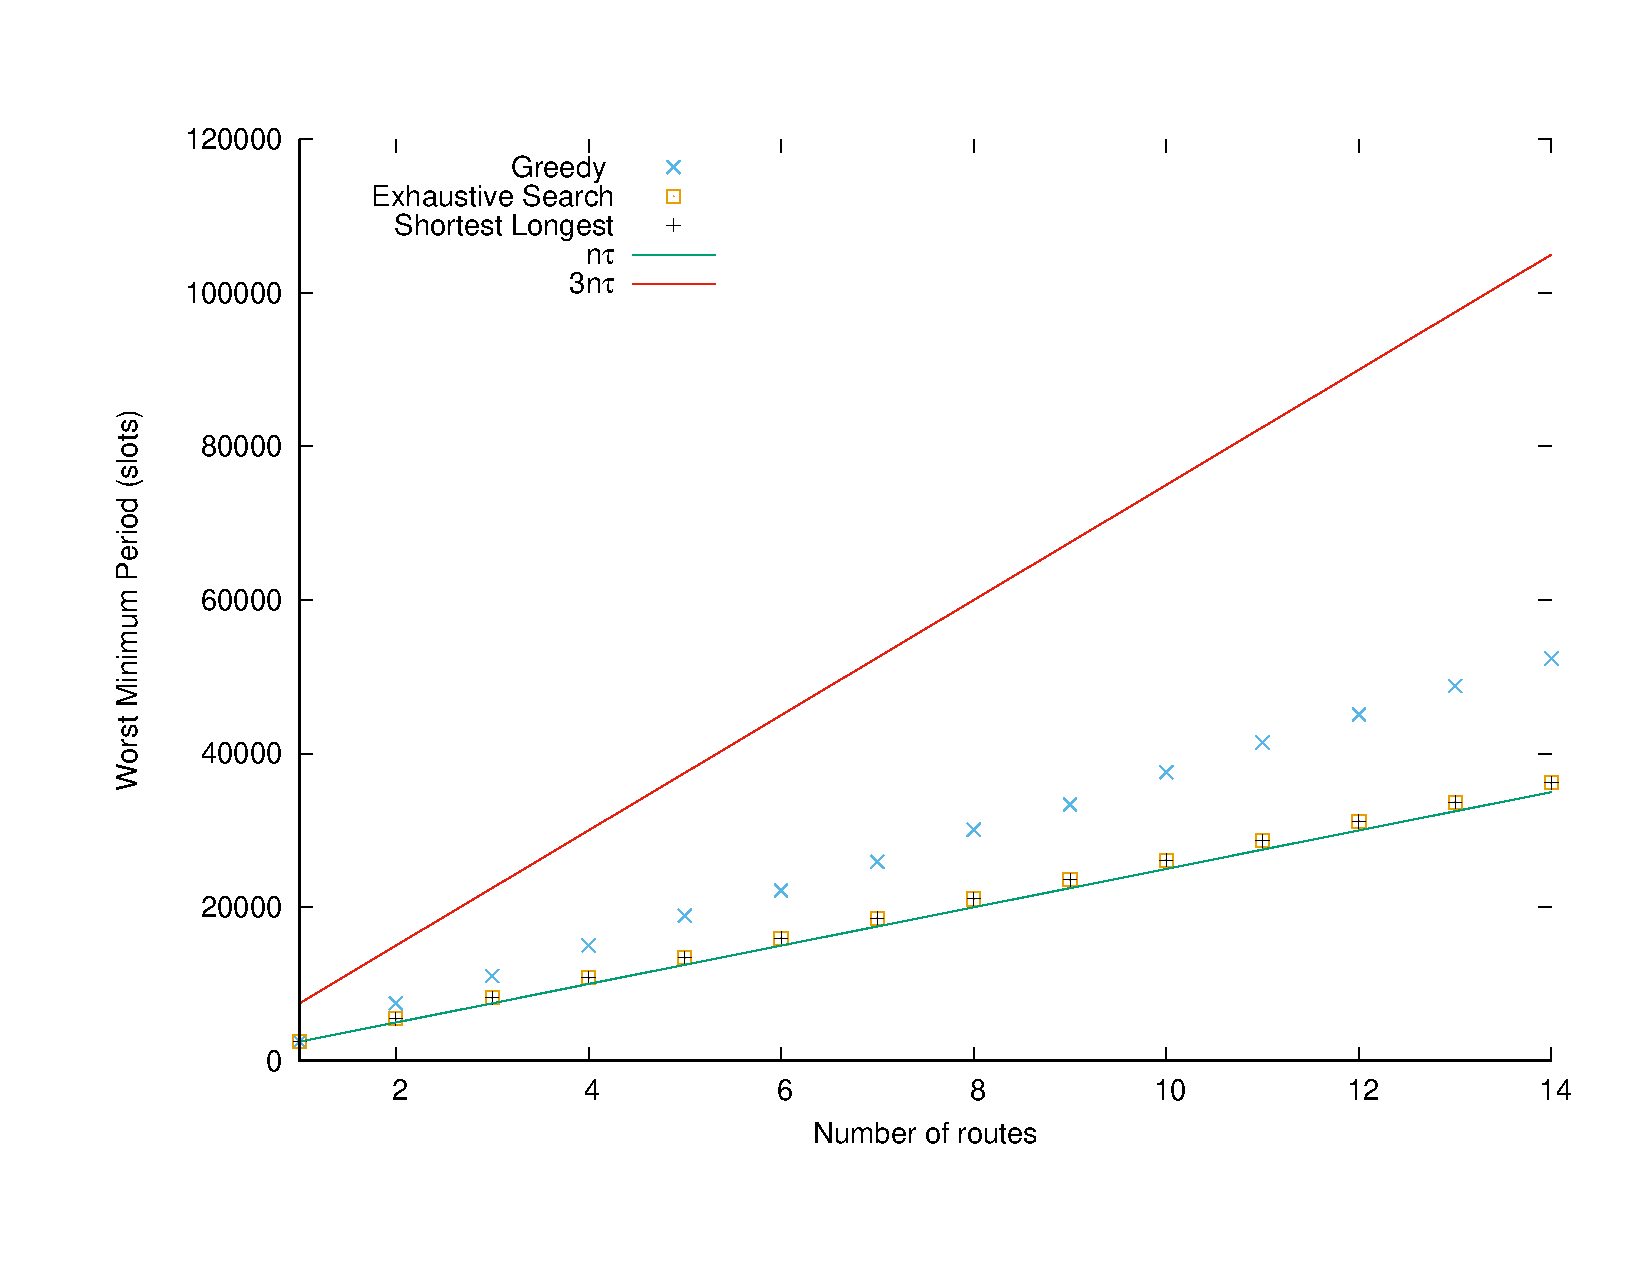
\includegraphics[width=0.47\textwidth]{periode_petite.pdf}
      \end{center}
      \caption{Minimum period averaged over $1,000$ random instances}\label{fig:short}
      \end{figure}
      First, we remark that the exhaustive search finds a solution even when the load is high, especially when there are more routes.
      It justifies the idea to look for an assignment without waiting time, in this short routes regime.
      Second, remark that the Shortest-Longest algorithm is as good as the exhaustive search. While it was expected to be good with short routes, it turns out to be optimal for all the the random star routed networks we have tried. Therefore, we should use it in practical applications with short routes, instead of the exhaustive search which is much more computationally expensive. 
      Finally, note that the greedy algorithm works on average when the load is less than $2/3$ which is twice better than the theoretical bound. This algorithm seems to depends on the load only and not on the number of routes.
      
        \paragraph{Long routes}
      
      We now want to understand the performance of these algorithms when the size of the routes is unbounded. In this experiment we fix the number of routes to $8$ and the weights of the arcs $(c_t,t_i)$ are drawn following an uniform distribution between $0$ and $20,000$ slots (in the same range as the period). We represent in Fig.~\ref{fig:long} the percentage of success of each algorithm, for load from $100\%$ down to $40\%$.
      
\begin{figure}[h]

       \begin{center}
      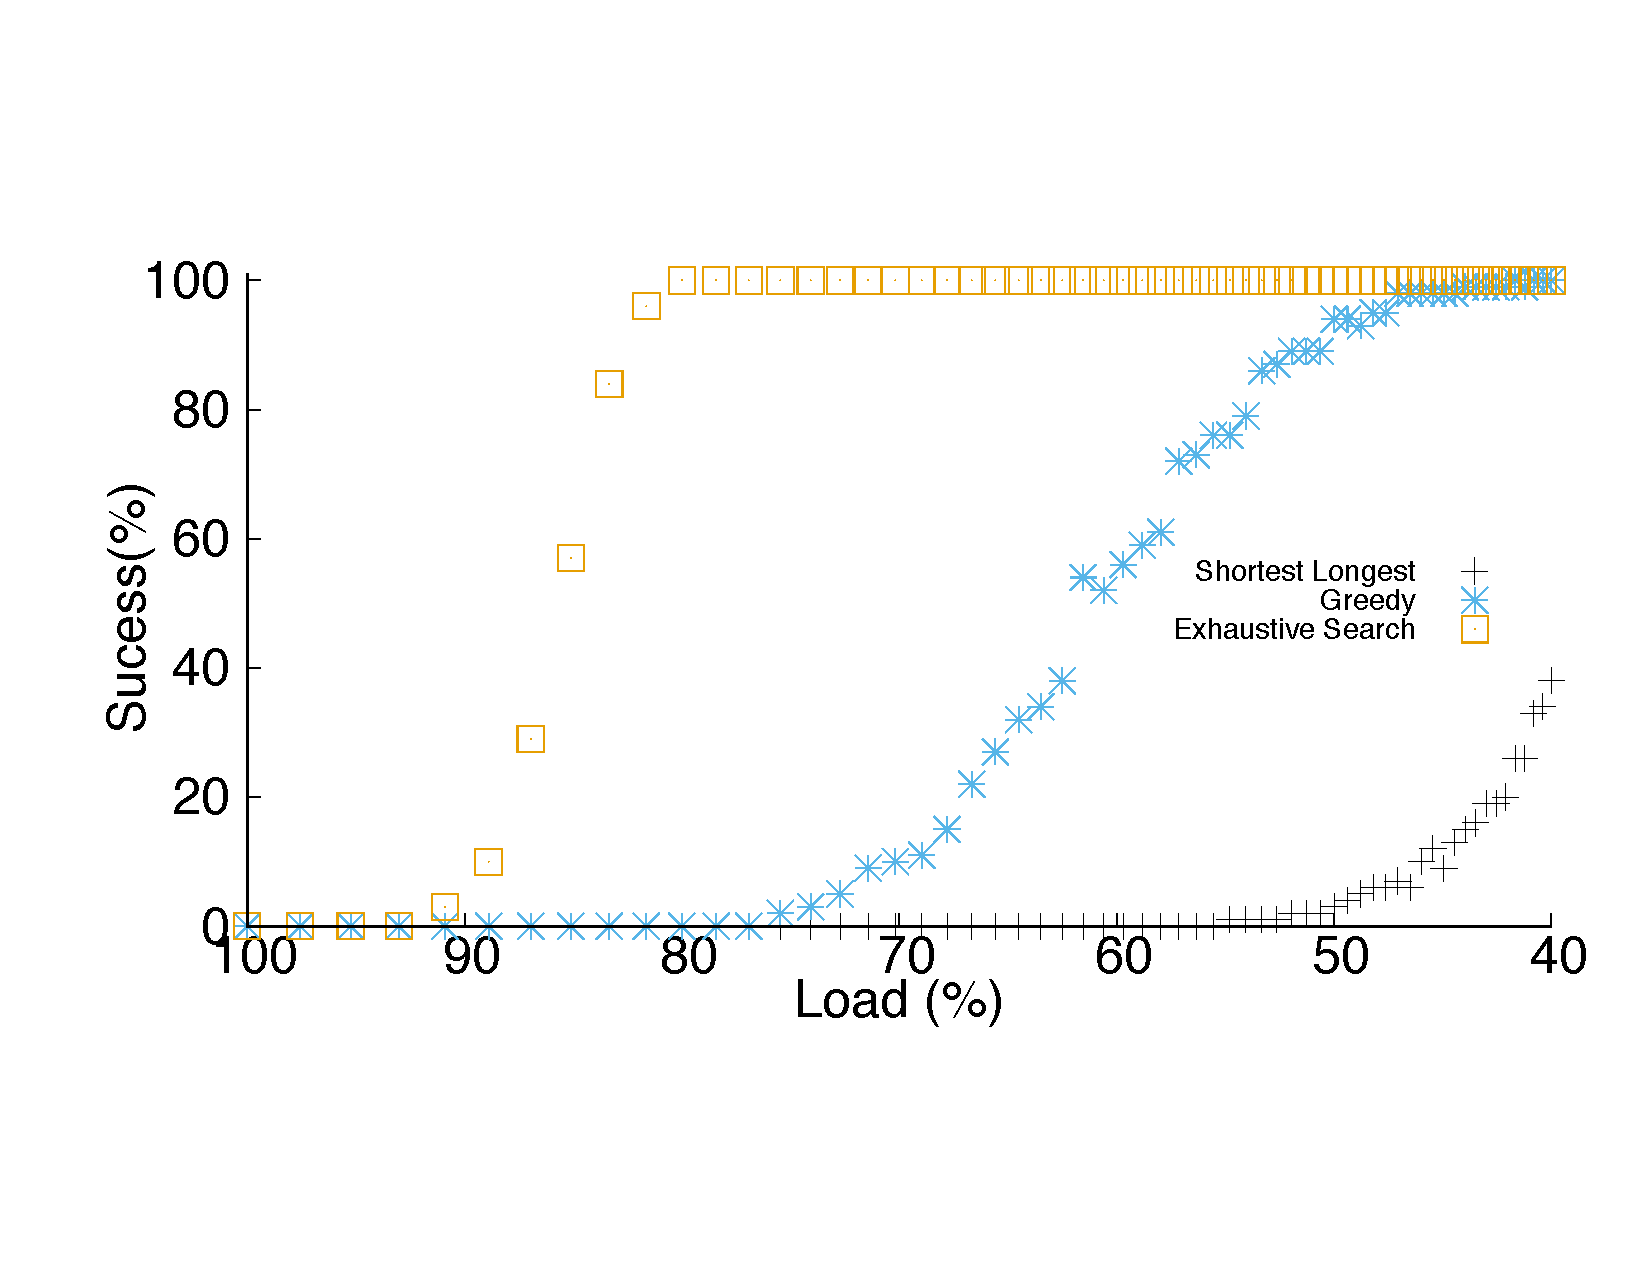
\includegraphics[width=0.47\textwidth]{echec_longues.pdf}
      \end{center}
       
      \caption{Success rate for $8$ routes over $1,000$ random instances}\label{fig:long}
     \end{figure}
      
      In this regime, the performances of Shortest-Longest are abysmal since it depends on the difference between the longest and the smallest route which is large here. On the other hand, the greedy algorithm has a performance not so far from the case of short routes, which is expected since it does not directly depend on the size of the route. In fact, if we do the previous experiment 
      for short routes but with long routes, we find that, on average, the greedy algorithm finds a solution when the load is less than $59\%$.
      
      When the load is larger than $50\%$, the exhaustive search finds more solutions than the greedy algorithms which justifies its use. However, for load larger than $80\%$ there are many instances for which there are no solutions to \pazl.
      It means that with long routes and high load, looking for an assignment without waiting time is far too restrictive. That is why we present algorithms for the general \pall problem in our next section. We will test them on $8$ long routes and a load between $100\%$ and $80\%$ for which, as shown here, there are often no assignment without waiting times.
      
      The computation time of the exhaustive search is in $O(n!)$ as shown int Th.~\ref{th:FPT}, hence we need to study its scalability when $n$ grows. In the following experiment, the weights of the arcs $(c_t,t_i)$ are drawn following an uniform distribution between $0$ and $20,000$ slots. We chose  $95\%$ of load.
%       , that corresponds to loads of $\simeq 70\%$ (for $1$ route) to $\simeq 98\%$ (for 21 routes).
      The following table shows the time before the exhaustive search ends, for $8$ to $16$ routes, averaged on $100$ random star routed networks. This shows that for less than $15$ routes, which corresponds to all current topologies, the algorithm is efficient enough, but we should improve it further to work on more routes.
         \begin{center}
         \begin{tabularx}{0.5\textwidth}{|l|X|X|X|X|X|}
    \hline
   $n$ & $8$ & $10$& $12$&$14$& $16$\\
    \hline
   Time (s) & $6.10^{-5}$&$8.10^{-4}$&$2.10^{-2}$& $0.4$& $11$\\
    \hline
      \end{tabularx}
      \end{center}
      
         \section{Solving \pall on Star Routed Networks}\label{sec:PALL}
    
    In this section, we consider the more general \pall problem on star routed networks. It means that the messages can wait in the target vertices (BBUs) in order to find assignments which is not possible for \pazl. We allow the process time of the routes to be greater than twice the weights of the routes, but it should be less than $T_{max}$.

	\subsection{Special cases}
		
		
	Often in real networks, the length of the routes are not arbitrary and we may exploit that to solve \pall easily. For instance if all the weights on the arcs $(c_t,t_i)$ are the same, we can replace them all by $0$ and substract this weight to $T_{max}$. It corresponds to a situation where all the BBUs are in the same datacenter and have the same processing power.
	The assignment in that case is trivial, just send all messages so that they follow each other without gaps in the central arc. Since the arcs $(c_t,t_i)$ are of weight $0$, all messages will go through $(c_t,c_s)$ on their way back in
	the same order and thus do not collide. 
	
 %A more realistic assumption would be that all weigths of the arcs $(s_i,c_s)$ are the same. It would correspond to a situation where all the BBUs are in the same datacenter.
	Another possible assumption would be that all weights of the arcs $(s_i,c_s)$ are the same.
	
	 \begin{theorem}\label{th:asym}
	 Let $(G,{\cal R})$ be a star routed network with $n$ routes and let $P \geq n\tau$. If there is a constant $c$ such that $\forall i < n, \,\omega(s_i,c_s) = c$, then there is a $(P,\tau)$-periodic assignment with process time $2\, \displaystyle{\max_{r\in {\cal R}} \lambda(r)}$.
% 	 and it can be built in time $O(n)$.
	 \end{theorem}
      \begin{proof}
      
        We can simplify the weights on the arcs $(s_i,c_s)$ by setting them all to $0$.
        We find the route with maximal length, say that it is $\lambda(r_0)$. The idea is to 
        set the waiting times of all routes so they behave exactly as the message in $r_0$.
        
        The offset of the forward route $r_i$ is set to $i\tau$, which ensures that there are no collision on the arc $(c_s,c_t)$ as soon as $P \geq n\tau$ which is the minimal possible period. We set the waiting time for the route $i$ to $w_i = 2(\lambda(r_{0}) - \lambda(r_{i}))$. We can compute the time at which the message of the route $r_i$ arrives at the vertex $c_t$ on its way back: $t(c_t,\rho(r_i)) = w_i + i\tau + 2\lambda(r_{i})$
        by replacing $w_i$ by its value we obtain $t(c_t,\rho(r_i)) =  i\tau + 2\lambda(r_{0})$
        As a conclusion there are no collision on the arc $(c_t,c_s)$ as soon as the 
        period is larger than $n\tau$ (there are no gaps between the messages).
        The process time of the route $r_i$ defined by $PT(r_i) = w_i + 2\lambda(r_{i}) $. We obtain $PT(r_i) = 2\lambda(r_{0})$ and thus the maximum process time of the assignment is also equal to $2\lambda(r_0)$.
% 	Finally the complexity is $O(n)$ since we have to find the maximum of the length of the $n$ routes and the computation of each $w_i$ is done by a constant number of arithmetic operations.
     \end{proof}
     
     Assume that for any pair of indices $(i,j)$ the difference between the weights of the arcs $(s_i,c_s)$ and $(s_j,c_s)$ is bounded by $d$ and the length of the longest route is $l$. Using the same idea as in Th.~\ref{th:asym}, there is an assignment with maximum process time bounded by  $2l + d$
     
     
%     We tried the five following orders. 
%	\begin{itemize}
%	 
%	 \item Longest-Shortest on Routes (LSR): Decreasing order on the length of the routes.
%	 \item Shortest-Longest on Routes (SLR): Increasing order on the length of the routes. 
%	 \item Longest-Shortest on last Arc (LSA): Decreasing order on the length of the arcs $(c_t,t_i)$.
%	 \item Shortest-Longest on last Arc (SLA): Increasing order on the length of the arcs $(c_t,t_i)$. This sending order yields a $(P,\tau)$ periodic assignment in which all the $w_i = 0$, if the period is large enough (see proposition \ref{prop:SL}).
%	 \item Random: A random order of the routes.
%	\end{itemize}
% 
%    In the rest of the section we will study different methods to compute the offsets of the backward routes, once
%    the offsets of the forward routes are fixed by one of the previous orders.
%    
   \subsection{Greedy scheduling of backward routes}
    
    We can decompose any algorithm solving the \pall problem in two stages: first set the offsets of the forward routes and then, knowing this information set the offset of the backward routes or equivalently the waiting times.  
    The offsets of the forward routes are chosen so that they have no collisions and such that there are no free slots in between the end of a message on the central arc and the beginning of the next one. 
    It is done to minimize the period needed to send the messages of the forward routes. For this section and the next, we assume that the offsets of the forward routes are fixed by some order. 
    
    Consider a forward route $r_i$ and the corresponding backward route $\rho(r_i)$.
    We define the {\bf deadline} of $\rho(r_i)$ as $m_{r_i} + T_{max} - \omega(s_i,c_s)$, that is the latest time at which the message can go out of $c_t$ such that $PT(r_i) \leq T_{max}$.
    We say that a backward route $\rho(r_i)$ is {\bf eligible} at time $t$ if $m_{i} +  \lambda(r_i) + \omega(c_t,t_i) \leq t$, that is the message of the route $\rho(r_i)$ arrives at $c_t$ before time $t$ when $w_i = 0$.
    
    The first algorithm we propose is a greedy algorithm which sets the offset $m_{\rho(r_i)}$ of the 
    backward routes. It prioritizes the routes with the earliest deadline to best satisfy the
    constraint on the process time. Set $t=0$ and repeat the following: find $s \geq t$ the first time for which there is an eligible route with its offset not fixed. Then amongst all eligible routes at time $s$ choose the one with the smallest deadline, fix its offset to $s - \omega(c_t,t_i) $ and set $t = s + \tau$.
    
    This algorithm does not take into account the periodicity. Say that $t_0 = t(c_t,r)$ such that $r$ is the first backward route selected by the algorithm. Then if all backward routes $r$ are such that $t(c_t,r)$ is smaller than $t_0 + P - \tau$,
    by construction, there are no collisions on the central arc.
    However, if a route $r$ has a larger $t(c_t,r)$, since we should consider everything modulo $P$, 
    it may collide with another backward route. Therefore we must adapt the greedy algorithm of the previous paragraph by finding $s \geq t$ the first time for which there is an eligible route with its offset not fixed and \emph{such that there is no collision if a message go through the central arc at time $s$}. 
    
%     
%      \begin{algorithm}
%     \caption{ Greedy deadline ({\bf GD}) }
%     \begin{algorithmic}
%     \REQUIRE A routed network $(G,{\cal R})$, a period $P$, packet size $\tau$, $ T_{max}$, the offsets $m_i$
%     \ENSURE $(P,\tau)$-periodic assignment of $(G,{\cal R})$, or failure
%    \STATE  ${\cal H} \leftarrow$ empty set //{\em set of eligible routes}
%        \STATE  free\_ intervals $\leftarrow$ [0,$P$] //{\em list of intervals of free slots}
%   
%     \FORALL{route $r_{i}$}
%     \STATE  deadline[$r_i$]  $\leftarrow$  $m_{i} + T_{max} - \omega(s_i,c_s)$
%     \STATE  eligible\_time[$r_i$] $\leftarrow$ $m_{i} +  \lambda(r_i) + \omega(c_t,t_i)$
%       \ENDFOR
%       
%       \WHILE{There is some non-assigned routes}
%       \IF{${\cal H}$ is empty}
%       \STATE $r_i$ $\leftarrow $ min\_non\_assigned(eligible\_time)
%       \ENDIF
%      
%       \STATE $r \leftarrow $ extract\_min(${\cal H}$)
%       \STATE t $\leftarrow$ next\_free\_interval(free\_intervals, t) //{\em if there is no more free intervals of size $\tau$, the algorithm fails}
%       \STATE $w_i \leftarrow$ t - eligible\_time[$r_i$]
%       \STATE update(t,free\_ intervals)
%       \STATE t $\leftarrow$ t + $\tau$
%       \FORALL{routes $r_i$ with  eligible\_time[$r_i$] $\leq$ t}
%       \STATE insert ( ${\cal H}$,$r_i$).
%       \ENDFOR
%       \ENDWHILE
% %    \STATE  $w_i \leftarrow 0$
% %    \FORALL{route $r_{t_i}$}
% %    \STATE  $w_i \leftarrow 0$
% %    \STATE period-end $\leftarrow m_{s_i} + \lambda(r_{s_i}) + t(c_t,r_{t_i}) + P$
% %    \FORALL{route $r_{t_j}$}
% %    \STATE deadline-route$ \leftarrow m_{s_j} + T_{max}-t(c_s,r_{s_j})$
% %    \STATE $deadline \leftarrow$ min(deadline-route,period-end)
% %    \ENDFOR
%     
% 
%     \end{algorithmic}
%     \end{algorithm}
%     The function  min\_non\_assigned(eligible\_time) returns the route with lowest time in eligible\_time, which is not assigned yet. The function update(t,free\_intervals) removes an interval of size $\tau$ beginning at t, which correspond to the message,  from free\_intervals.


    The greedy algorithm can be made to work in time $O(n\log(n))$ by using a binary heap for the set of eligible routes, and a list to maintain a list of the intervals
    of time at which a message can be sent on the arc $(c_t,c_s)$.
%    To do that the set of eligible routes must be maintained in a binary heap
%    to be able to find the one with smallest deadline in time $O(\log(n))$. 
%    To deal with the possible collisions, one can maintain a list of the intervals
%    of time at which a message can be sent on the arc $(c_t,c_s)$. Each time the offset of a 
%    route is fixed an interval is split into at most two intervals in constant time. 
%    Since the algorithm goes over the elements of the list at most twice when doing an insertion
%    or looking for the next free interval, the time needed to maintain it is $O(n)$. 
%    
%     
%          We compared the two algorithms on $10000$ graphs on which the weight of the links are drawn uniformly between $0$ and $20000$, with a period of $21000$, and giving, for each instance $T_{max} = 2\lambda(r_{longest-route})$ . We then look at the success rate of each algorithms, with every sending order. Both algorithms reach the higher success rate with the Random sending order, but the success of Greedy is $5,65 \%$, while the success rate of Greedy Periodic is to $30,02 \%$.
    

    
     
     \subsection{Earliest deadline scheduling}
     
     
     The problem to solve in the second stage of our approach is very similar to the following scheduling problem: 
     we are given a set of jobs and each job has a \emph{release time} and a \emph{deadline}. 
     The problem is to schedule all jobs on a single processor, that is choosing the time at which they are computed, so that no two jobs are scheduled at the same time. A job is always scheduled after its release time and it must be finished before its deadline. Let us call $n$ the number of jobs, the problem can be solved in time $O(n^2\log(n))$~\cite{simons1978fast} when all jobs have the same running time and it gives a solution with the earliest possible deadline. On the other hand if the running times are different the problem is $\NP$-complete~\cite{lenstra1977complexity}. 
     The  polynomial time algorithm  which solves this scheduling problem is similar to the Greedy algorithm presented in the previous section. However, when it fails because a job finishes after its deadline, it changes the schedule of the last messages to find a possible schedule for the problematic job. The change in the scheduling is so that the algorithm cannot fail on the same job a second time except if there is no solution, which proves that the algorithm is in polynomial time.
     
     We reduce our problem of setting the offsets of the backwards routes once the order of the forward routes is fixed to this
     scheduling problem. The backward routes are the jobs, the size of a message is the running time of a job,
     the deadline of a route is the deadline of the corresponding job and the smallest time at which it is eligible is the release time. Let us call {\bf Minimal Latency Scheduling (MLS)} this algorithm.
     Remark that we do not deal with the periodicity. When MLS finds an assignment $m$ its always satisfies $MPT(m) < T_{max}$. On the other hand, it is a $(P,\tau)$ periodic assignment only if $m_{max} - m_{min} \leq P -\tau$ where $m_{max}$ is the largest offset and $m_{min}$ the smallest one. The algorithm we use minimize this quantity, so it may work in practice (as shown in Section~\ref{sec:resultsPALL}).
     
     We now present a variant of the previous algorithm that we call {\bf Periodic Minimal Latency Scheduling (PMLS)}
     which takes into account the periodicity. We fix arbitrarily a backward route so that its message is the first to go through the central arc at time $t$. Then we modify the deadline of each backward route to be the minimum of their previous deadline and $t + P$.  We execute this algorithm for every possible first backward route and we return the solution that minimizes $MPT(m)$. Since we run the previous algorithm at most $n$ times, the complexity is in $O(n^3\log(n))$. Remark that it finds an assignment more often than MLS, because if MLS finds a solution with first route $r$ and such that $m_{max} - m_{min} \leq P -\tau$, then this solution will be found by PMLS when it selects $r$ as the first route. Moreover when PMLS finds a solution, it is always a $(P,\tau)$ periodic assignment since we guarantee that all messages are scheduled in a period of time of size $P$ and it satisfies $MPT(m) < T_{max}$ by construction of the deadlines. Remark that PMLS may fail while there is an assignment. Indeed, in the algorithm we restrict the assignments we look for by not allowing to choose an offset for a route after $t+P- \tau$.
     
%     \begin{algorithm}[H]
%     \caption{ Minimized Scheduling Periodic (MSP)}
%     \begin{algorithmic}
%     \REQUIRE A routed network $(G,{\cal R})$,a period $P$, packet size $\tau$, $ T_{max}$, the offsets $m_i$
%     \ENSURE $(P-\tau)-$periodic assignment of $(G,{\cal R})$, if it exists
%   
%     \FORALL{route $r_{t_i}$}
%     \STATE  $w_i \leftarrow 0$
%     \STATE period-end $\leftarrow m_{s_i} + \lambda(r_{s_i}) + t(c_t,r_{t_i}) + P$
%     \FORALL{route $r_{t_j}$}
%     \STATE deadline-route$ \leftarrow m_{s_j} + T_{max}-t(c_s,r_{s_j})$
%     \STATE $deadline \leftarrow$ min(deadline-route,period-end)
%     \ENDFOR
%     
%     \STATE Call (MS)
% 
%     
%     \ENDFOR
% 
%     \STATE return the best $(P,\tau)$-periodic assignment, or FAILURE
% 
%     \end{algorithmic}
%     \end{algorithm}
    \subsection{Experimental evaluation}
    \label{sec:resultsPALL}
    
    We fix the number of routes to $8$ to make comparisons with the results of Section~\ref{sec:exp_PAZL} easier. 
    We draw uniformly the weights of the arcs between $0$ and $20,000$.
    For a given routed network, we define the {\em margin} as the difference between $T_{max}$ and twice the longest route. 
    Hence, for a given routed network choosing the margin or $T_{max}$ is the same, but since we will consider many networks with different longest route's size, it will be more meaningful to set a global margin rather than $T_{max}$.
    In fact the margin represents the latency imposed by the communication process without taking into account the physical length of the network which cannot be changed. In our experiments the margin range from  $0$ to $3,000$.
   We look at two different regimes, a medium load of $80\%$ and a high load of $95\%$.
   Considering smaller load is not relevant since then we know how to solve the problem even without waiting times as shown in Section~\ref{sec:exp_PAZL}. 
   
   We first try to understand what is the best choice of order for the first stage of the algorithm which is followed by the GD algorithm in this experiment. We try the following ones: decreasing order on the length of the routes (LSR), decreasing order on the weigths of the arcs $(c_t,t_i)$ (LSA), increasing order on the length of the routes (SLR), increasing order on the weigths of the arcs $(c_t,t_i)$ (SLA). We also consider the random order, which means we compute $1,000$ random orders and stop as soon one yields an assignment.
   In Fig.~\ref{fig:success95} , we represent the success rate of the five kind of orders with regards to the margin. The value is an average computed over $10,000$ random star routed networks.

\begin{figure}[h] 
  \centering
    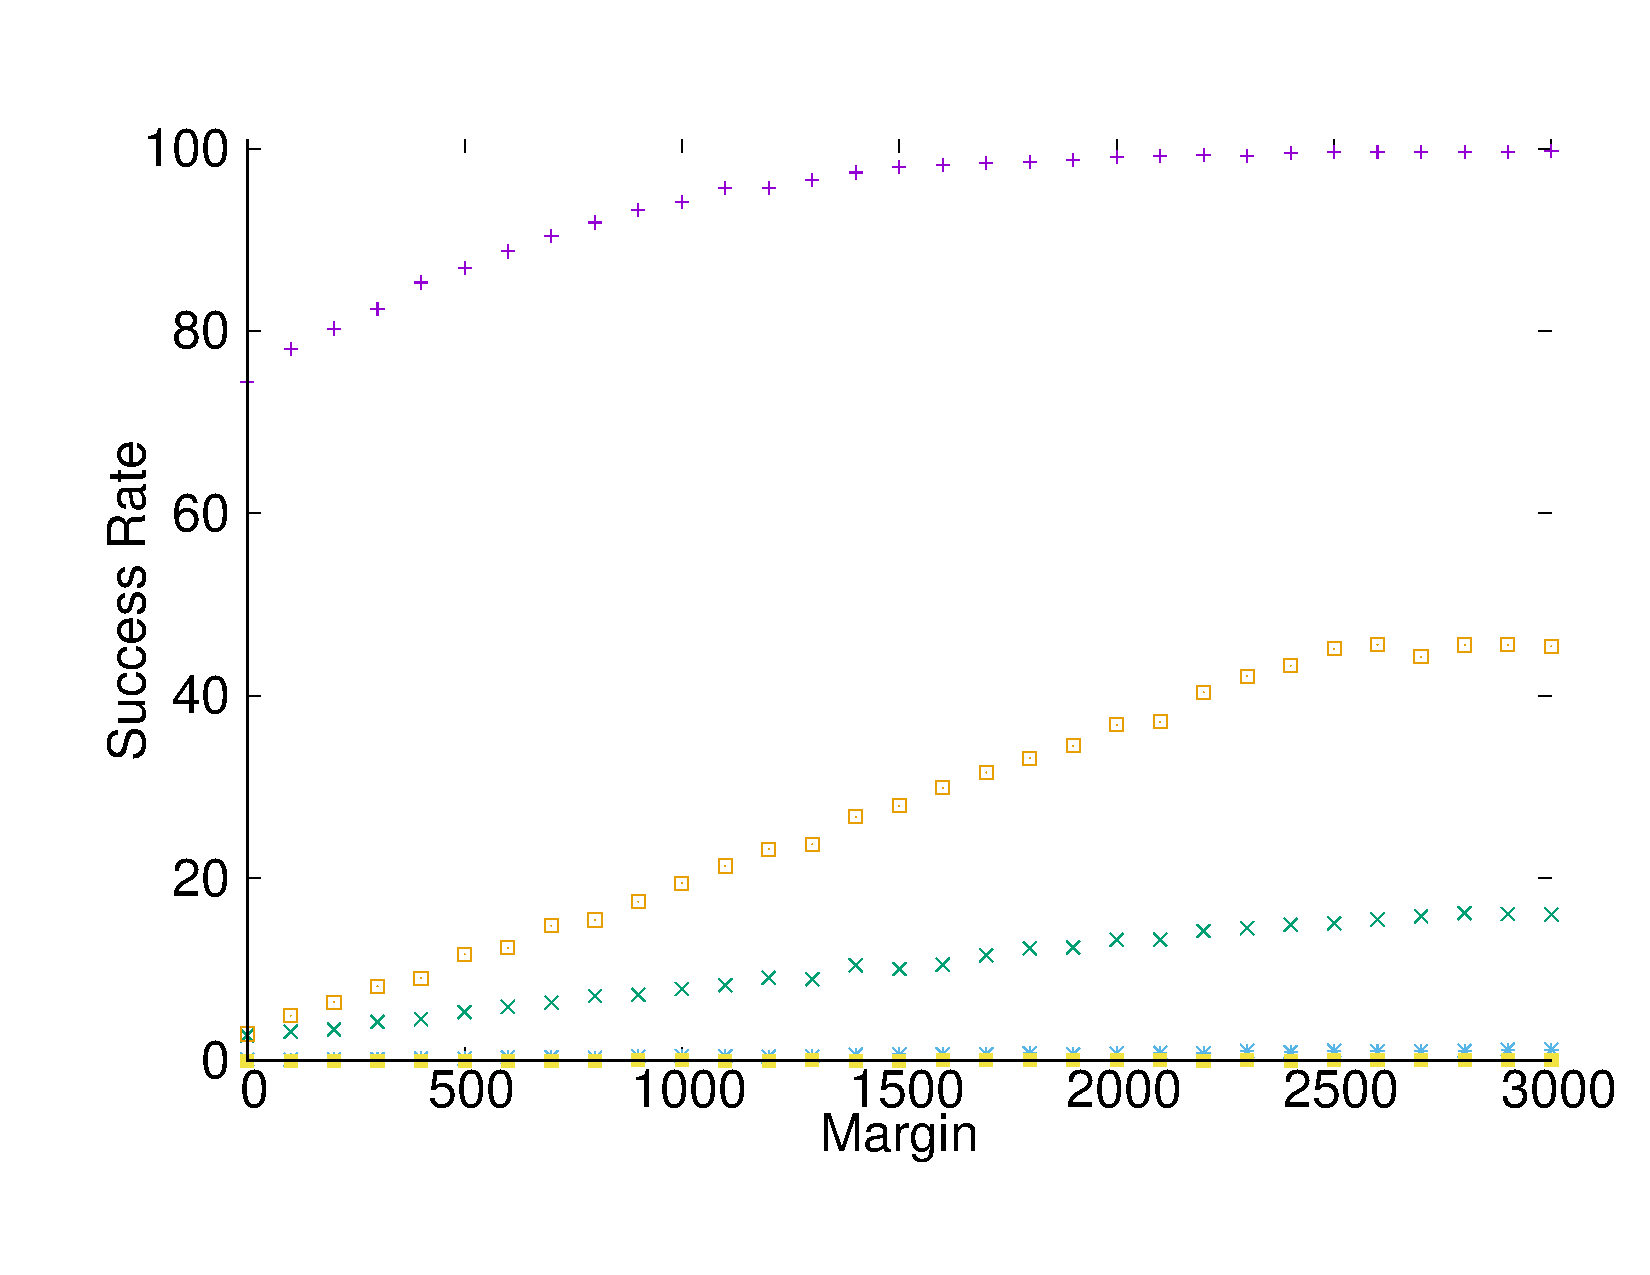
\includegraphics[width=0.5\textwidth]{departs_gp_21000.pdf}
      \caption{Success rate of different orders, $95\%$ load.}
      \label{fig:success95}
          \end{figure}

%\begin{figure}[h] 
%          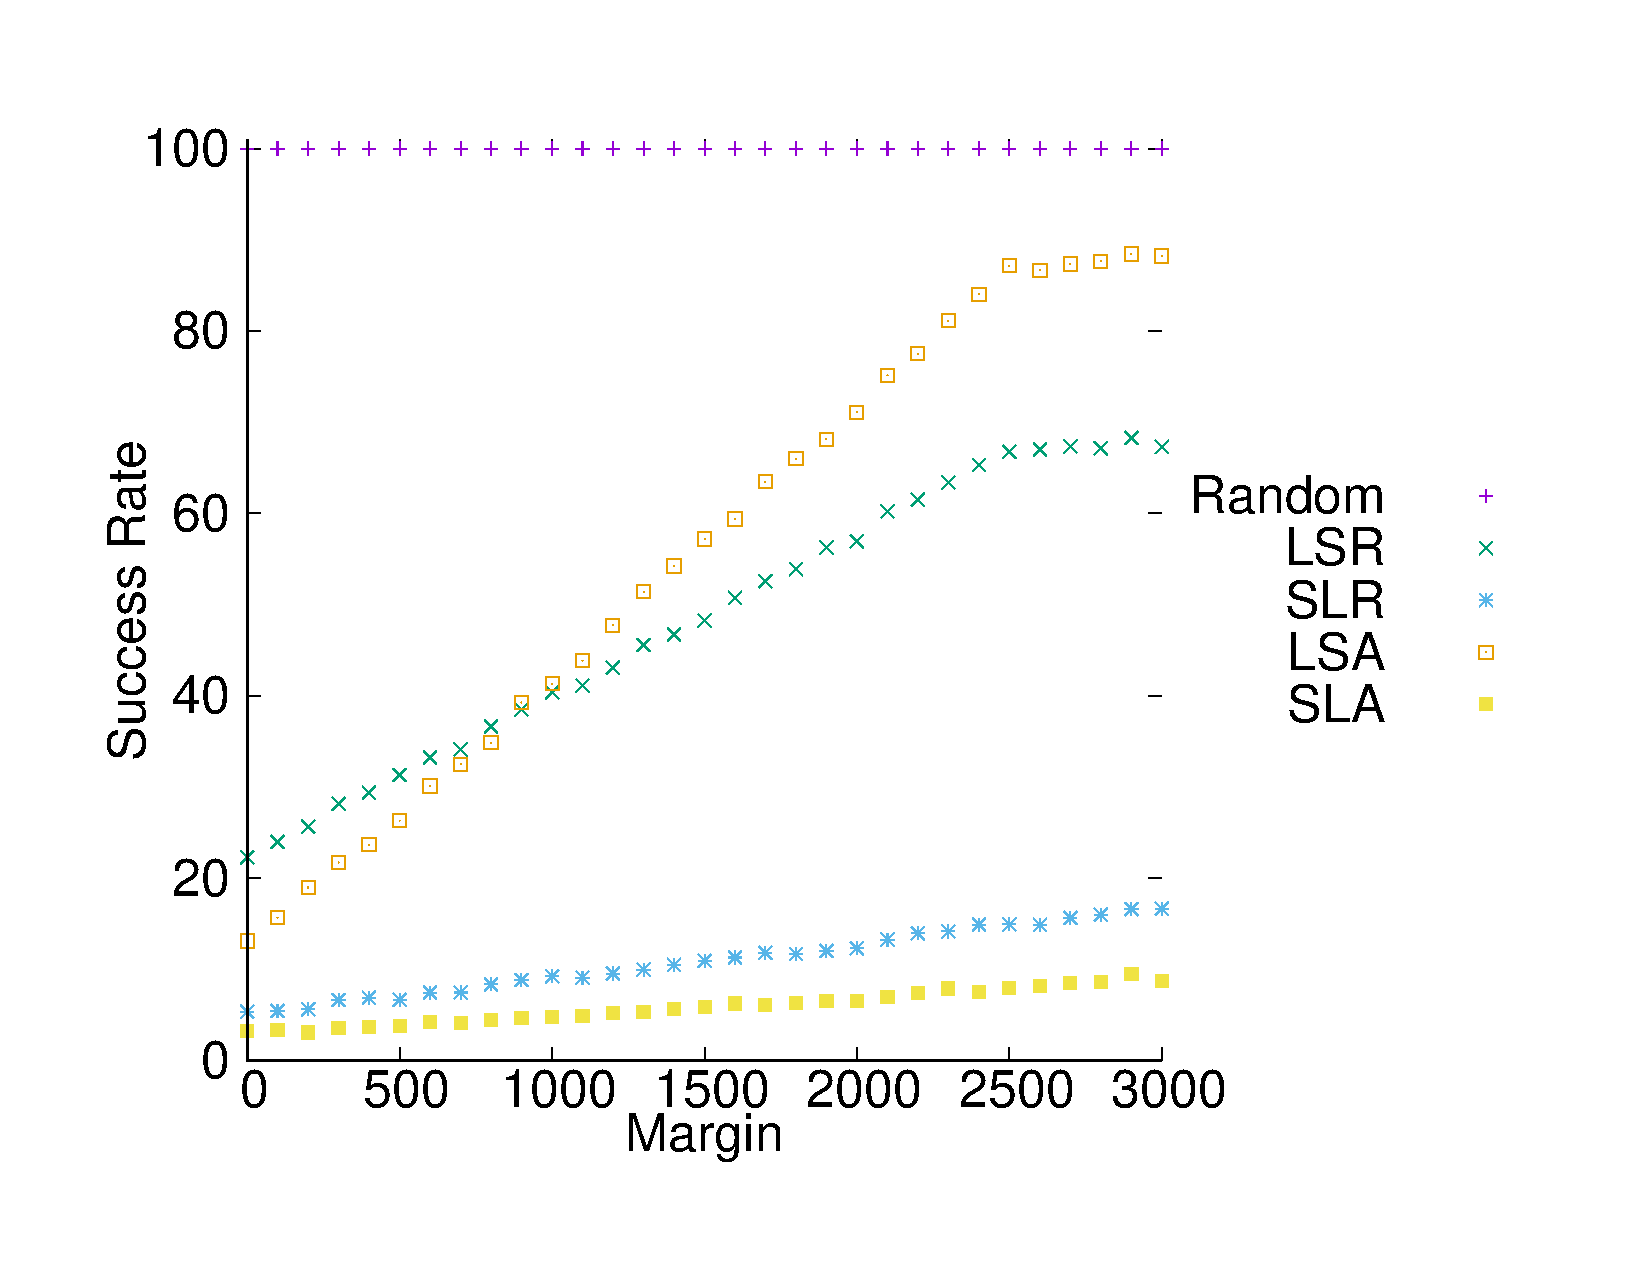
\includegraphics[width=0.4\textwidth]{departs_gp_25000.pdf}
%          \vspace{-0.5cm}
%      \caption{Success rate of different orders, $80\%$ load.}
%           \label{fig:success80}
%     \end{figure}
     
     According to our experiments, sending the messages from the shortest to the longest route or arc does not work well. It corresponds to the policy of Prop.~\ref{prop:SL} which we already know to be bad for \pazl when the routes are long as in this experiment. Sending from the longest to the shortest route or arc works better and it seems that sorting the routes according to the length of the last arc rather than the route is better, at least in a loaded network. 
     
     The random order is the best by far: with a load of $95\%$, there is solution with margin $0$ most of the time. Note that, when disallowing waiting times, there were no instances with an assignment for these parameters (see Section~\ref{sec:exp_PAZL}), which justifies the interest of studying the \pall problem. We now want to compare the performances of the three different algorithms used in the second stage. Since GD already showed excellent results on mild loads, it is more interesting to focus on the behavior of the algorithms on high load. Moreover, we will use $1,000$ random orders for the first stage as it gives the best results. In the following experiment, we represent the success rate of the three algorithms with regards to the margin,  computed over $10,000$ random star routed networks and the same parameters as previously.
     
    \begin{figure} [h] 
       \begin{center}
      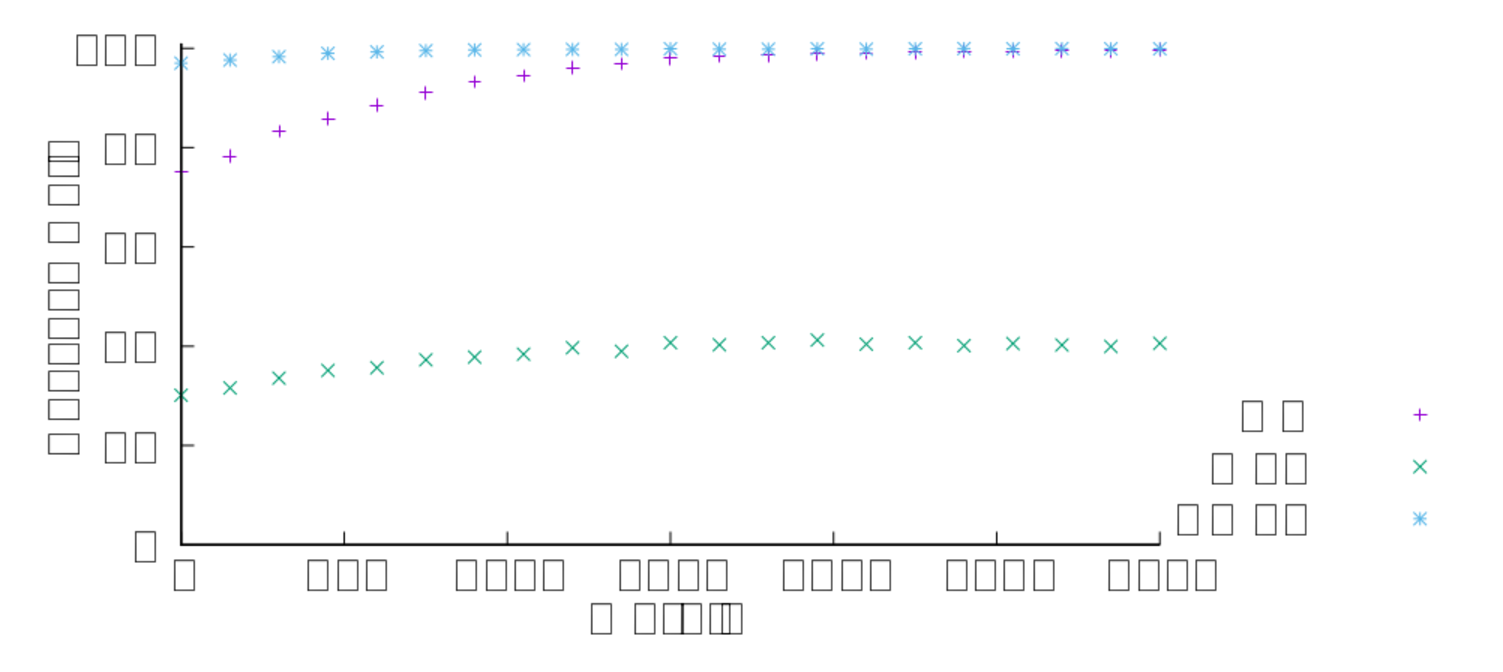
\includegraphics[width=0.5\textwidth]{retour_21000.pdf}
      \end{center}
      \caption{Success rate of GD, MLS and PMLS, $95\%$ load}
     \label{fig:success21000}
     \end{figure}

     The MLS algorithm performs poorly, worst than GD and PMLS, which shows that \emph{taking into account the periodicity is fundamental}.
     The GD algorithms is close to $100\%$ success rate for margins larger than $1,500$ while the PMLS algorithm finds a solution in more than $97\%$ of the experiments, even with a margin $0$. Therefore, for the worst possible constraints on load and margin, there are a few instances for which we do not find a solution. However, with a margin of $1,000$, which corresponds to about $0.05$ms of additional delay with the chosen parameters, we always find a solution. 
     
    Recall that the random order corresponds to the best of $1,000$ orders drawn uniformly which means that a computation can be up to $1,000$ time slower than for a fixed order. The choice of the number of random orders drawn yields a trade-off between the computation time and the success rate. Up to now, we chose $1,000$ random orders arbitrarily. We investigate the success rate of our algorithm with regards to the number of random orders drawn, a load of $95\%$ and a margin $0$. The following tables presents the average success rate for each number of sending orders, on $10,000$ instances, for GD and PMLS.
         \begin{figure}[h] 
       \begin{center}
   \begin{tabularx}{0.5\textwidth}{|c|X|X|X|X|X|X|}
    \hline
    \# orders& $1$ & $10$ & $100$& $1,000$& $10^{4}$&$10^{5}$\\
    \hline
    GD & $0.6$ &$7.1$&$33.4$&$76.4$&$90.0$&$90.0$\\
    \hline
  PMLS & $38.9$ &$83.0$&$95.3$&$97.2$&$97.5$&$97.7$\\
    \hline
      \end{tabularx}
      \end{center}
   \caption{Impact of the number of random sending orders}
     \end{figure}

First remark that we can improve our previous results by taking $10,000$ random orders,
instead of $1,000$. The number of different orders is $7!= 5,040$ since we have $8$ routes and the solutions are invariant up to a circular permutation of the order. Therefore instead of doing $10,000$ random draws we could test every possible order in less time. However the computation time of this method would scale badly with $n$. On the other hand, remark that the success rate of PMLS is already high for $100$ random orders, which means it will work even better than the other methods when $n$ is larger and that the number of random orders drawn becomes critical.
     
     
     
     Now that we have found the best amongst the algorithms solving \pall, we need to compare its performances against the actual way to manage the messages in a network:  statistical multiplexing, where there is a FIFO buffer in each node of the network to deal with the collisions. The time at which the messages are sent in the network is not computed as in our approach, thus we fix the offsets of each route to some random value.
     Even if this policy seems to work in practice when the network is not too loaded, it does not give any guarantee on the latency. Remark that the process is not periodic, therefore we must measure the process time of each route over several periods if we want to compute its maximum. We choose to simulate it for $1,000$ periods and we have observed that the process time usually stabilizes after $10$ periods. The margin is defined as the maximum process time, computed as explained, minus twice the size of the longest route. 
	    
     
     We draw $1000$ star routed networks with $8$ routes, with weights on the arcs drawn between $0$ and $20,000$. Note that the results are almost the same when the arcs are small. We measure, for load from $100\%$ down to $40\%$, the median, the first, and the third quartile of the margins computed in $1,000$ simulations using FIFO buffer to resolve collisions.

      
    \begin{figure}
       \begin{center}
      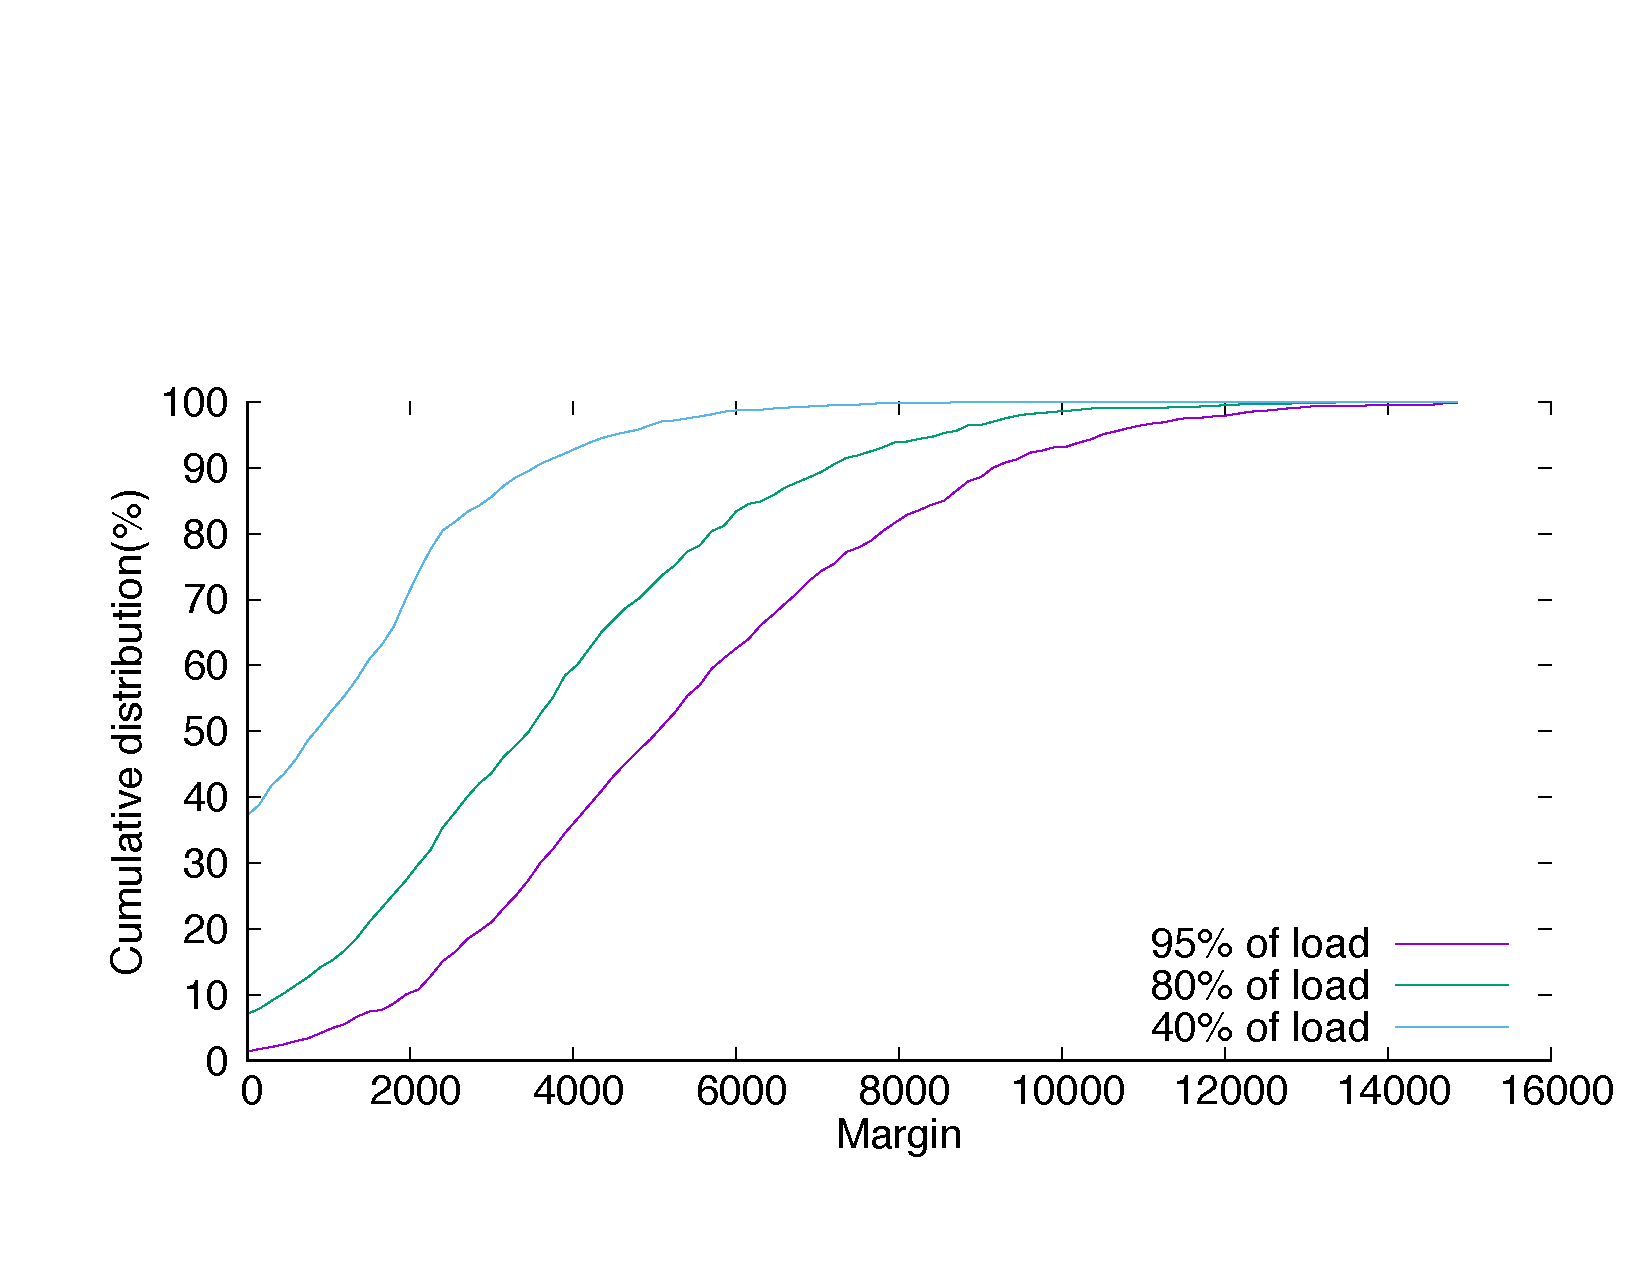
\includegraphics[width = 0.45\textwidth]{stochastic.pdf}
       %% GNUPLOT: LaTeX picture
\setlength{\unitlength}{0.240900pt}
\ifx\plotpoint\undefined\newsavebox{\plotpoint}\fi
\sbox{\plotpoint}{\rule[-0.200pt]{0.400pt}{0.400pt}}%
\begin{picture}(1500,900)(0,0)
\sbox{\plotpoint}{\rule[-0.200pt]{0.400pt}{0.400pt}}%
\put(171.0,131.0){\rule[-0.200pt]{4.818pt}{0.400pt}}
\put(151,131){\makebox(0,0)[r]{$0$}}
\put(1279.0,131.0){\rule[-0.200pt]{4.818pt}{0.400pt}}
\put(171.0,212.0){\rule[-0.200pt]{4.818pt}{0.400pt}}
\put(151,212){\makebox(0,0)[r]{$1000$}}
\put(1279.0,212.0){\rule[-0.200pt]{4.818pt}{0.400pt}}
\put(171.0,293.0){\rule[-0.200pt]{4.818pt}{0.400pt}}
\put(151,293){\makebox(0,0)[r]{$2000$}}
\put(1279.0,293.0){\rule[-0.200pt]{4.818pt}{0.400pt}}
\put(171.0,374.0){\rule[-0.200pt]{4.818pt}{0.400pt}}
\put(151,374){\makebox(0,0)[r]{$3000$}}
\put(1279.0,374.0){\rule[-0.200pt]{4.818pt}{0.400pt}}
\put(171.0,455.0){\rule[-0.200pt]{4.818pt}{0.400pt}}
\put(151,455){\makebox(0,0)[r]{$4000$}}
\put(1279.0,455.0){\rule[-0.200pt]{4.818pt}{0.400pt}}
\put(171.0,535.0){\rule[-0.200pt]{4.818pt}{0.400pt}}
\put(151,535){\makebox(0,0)[r]{$5000$}}
\put(1279.0,535.0){\rule[-0.200pt]{4.818pt}{0.400pt}}
\put(171.0,616.0){\rule[-0.200pt]{4.818pt}{0.400pt}}
\put(151,616){\makebox(0,0)[r]{$6000$}}
\put(1279.0,616.0){\rule[-0.200pt]{4.818pt}{0.400pt}}
\put(171.0,697.0){\rule[-0.200pt]{4.818pt}{0.400pt}}
\put(151,697){\makebox(0,0)[r]{$7000$}}
\put(1279.0,697.0){\rule[-0.200pt]{4.818pt}{0.400pt}}
\put(171.0,778.0){\rule[-0.200pt]{4.818pt}{0.400pt}}
\put(151,778){\makebox(0,0)[r]{$8000$}}
\put(1279.0,778.0){\rule[-0.200pt]{4.818pt}{0.400pt}}
\put(171.0,859.0){\rule[-0.200pt]{4.818pt}{0.400pt}}
\put(151,859){\makebox(0,0)[r]{$9000$}}
\put(1279.0,859.0){\rule[-0.200pt]{4.818pt}{0.400pt}}
\put(171.0,131.0){\rule[-0.200pt]{0.400pt}{4.818pt}}
\put(171,90){\makebox(0,0){$20000$}}
\put(171.0,839.0){\rule[-0.200pt]{0.400pt}{4.818pt}}
\put(359.0,131.0){\rule[-0.200pt]{0.400pt}{4.818pt}}
\put(359,90){\makebox(0,0){$25000$}}
\put(359.0,839.0){\rule[-0.200pt]{0.400pt}{4.818pt}}
\put(547.0,131.0){\rule[-0.200pt]{0.400pt}{4.818pt}}
\put(547,90){\makebox(0,0){$30000$}}
\put(547.0,839.0){\rule[-0.200pt]{0.400pt}{4.818pt}}
\put(735.0,131.0){\rule[-0.200pt]{0.400pt}{4.818pt}}
\put(735,90){\makebox(0,0){$35000$}}
\put(735.0,839.0){\rule[-0.200pt]{0.400pt}{4.818pt}}
\put(923.0,131.0){\rule[-0.200pt]{0.400pt}{4.818pt}}
\put(923,90){\makebox(0,0){$40000$}}
\put(923.0,839.0){\rule[-0.200pt]{0.400pt}{4.818pt}}
\put(1111.0,131.0){\rule[-0.200pt]{0.400pt}{4.818pt}}
\put(1111,90){\makebox(0,0){$45000$}}
\put(1111.0,839.0){\rule[-0.200pt]{0.400pt}{4.818pt}}
\put(1299.0,131.0){\rule[-0.200pt]{0.400pt}{4.818pt}}
\put(1299,90){\makebox(0,0){$50000$}}
\put(1299.0,839.0){\rule[-0.200pt]{0.400pt}{4.818pt}}
\put(171.0,131.0){\rule[-0.200pt]{0.400pt}{175.375pt}}
\put(171.0,131.0){\rule[-0.200pt]{271.735pt}{0.400pt}}
\put(30,495){\makebox(0,0){Needed Flexibility}}
\put(735,29){\makebox(0,0){Period}}
\put(171.0,455.0){\rule[-0.200pt]{0.400pt}{81.183pt}}
\put(171.0,455.0){\rule[-0.200pt]{2.409pt}{0.400pt}}
\put(171.0,792.0){\rule[-0.200pt]{2.409pt}{0.400pt}}
\put(209.0,412.0){\rule[-0.200pt]{0.400pt}{73.715pt}}
\put(199.0,412.0){\rule[-0.200pt]{4.818pt}{0.400pt}}
\put(199.0,718.0){\rule[-0.200pt]{4.818pt}{0.400pt}}
\put(246.0,353.0){\rule[-0.200pt]{0.400pt}{79.497pt}}
\put(236.0,353.0){\rule[-0.200pt]{4.818pt}{0.400pt}}
\put(236.0,683.0){\rule[-0.200pt]{4.818pt}{0.400pt}}
\put(284.0,336.0){\rule[-0.200pt]{0.400pt}{75.883pt}}
\put(274.0,336.0){\rule[-0.200pt]{4.818pt}{0.400pt}}
\put(274.0,651.0){\rule[-0.200pt]{4.818pt}{0.400pt}}
\put(321.0,306.0){\rule[-0.200pt]{0.400pt}{70.343pt}}
\put(311.0,306.0){\rule[-0.200pt]{4.818pt}{0.400pt}}
\put(311.0,598.0){\rule[-0.200pt]{4.818pt}{0.400pt}}
\put(359.0,297.0){\rule[-0.200pt]{0.400pt}{73.715pt}}
\put(349.0,297.0){\rule[-0.200pt]{4.818pt}{0.400pt}}
\put(349.0,603.0){\rule[-0.200pt]{4.818pt}{0.400pt}}
\put(397.0,270.0){\rule[-0.200pt]{0.400pt}{63.598pt}}
\put(387.0,270.0){\rule[-0.200pt]{4.818pt}{0.400pt}}
\put(387.0,534.0){\rule[-0.200pt]{4.818pt}{0.400pt}}
\put(434.0,269.0){\rule[-0.200pt]{0.400pt}{64.561pt}}
\put(424.0,269.0){\rule[-0.200pt]{4.818pt}{0.400pt}}
\put(424.0,537.0){\rule[-0.200pt]{4.818pt}{0.400pt}}
\put(472.0,238.0){\rule[-0.200pt]{0.400pt}{69.138pt}}
\put(462.0,238.0){\rule[-0.200pt]{4.818pt}{0.400pt}}
\put(462.0,525.0){\rule[-0.200pt]{4.818pt}{0.400pt}}
\put(509.0,226.0){\rule[-0.200pt]{0.400pt}{62.393pt}}
\put(499.0,226.0){\rule[-0.200pt]{4.818pt}{0.400pt}}
\put(499.0,485.0){\rule[-0.200pt]{4.818pt}{0.400pt}}
\put(547.0,222.0){\rule[-0.200pt]{0.400pt}{60.225pt}}
\put(537.0,222.0){\rule[-0.200pt]{4.818pt}{0.400pt}}
\put(537.0,472.0){\rule[-0.200pt]{4.818pt}{0.400pt}}
\put(585.0,195.0){\rule[-0.200pt]{0.400pt}{60.225pt}}
\put(575.0,195.0){\rule[-0.200pt]{4.818pt}{0.400pt}}
\put(575.0,445.0){\rule[-0.200pt]{4.818pt}{0.400pt}}
\put(622.0,185.0){\rule[-0.200pt]{0.400pt}{58.780pt}}
\put(612.0,185.0){\rule[-0.200pt]{4.818pt}{0.400pt}}
\put(612.0,429.0){\rule[-0.200pt]{4.818pt}{0.400pt}}
\put(660.0,178.0){\rule[-0.200pt]{0.400pt}{59.743pt}}
\put(650.0,178.0){\rule[-0.200pt]{4.818pt}{0.400pt}}
\put(650.0,426.0){\rule[-0.200pt]{4.818pt}{0.400pt}}
\put(697.0,188.0){\rule[-0.200pt]{0.400pt}{59.020pt}}
\put(687.0,188.0){\rule[-0.200pt]{4.818pt}{0.400pt}}
\put(687.0,433.0){\rule[-0.200pt]{4.818pt}{0.400pt}}
\put(735.0,152.0){\rule[-0.200pt]{0.400pt}{55.889pt}}
\put(725.0,152.0){\rule[-0.200pt]{4.818pt}{0.400pt}}
\put(725.0,384.0){\rule[-0.200pt]{4.818pt}{0.400pt}}
\put(773.0,146.0){\rule[-0.200pt]{0.400pt}{57.575pt}}
\put(763.0,146.0){\rule[-0.200pt]{4.818pt}{0.400pt}}
\put(763.0,385.0){\rule[-0.200pt]{4.818pt}{0.400pt}}
\put(810.0,146.0){\rule[-0.200pt]{0.400pt}{54.925pt}}
\put(800.0,146.0){\rule[-0.200pt]{4.818pt}{0.400pt}}
\put(800.0,374.0){\rule[-0.200pt]{4.818pt}{0.400pt}}
\put(848.0,143.0){\rule[-0.200pt]{0.400pt}{56.371pt}}
\put(838.0,143.0){\rule[-0.200pt]{4.818pt}{0.400pt}}
\put(838.0,377.0){\rule[-0.200pt]{4.818pt}{0.400pt}}
\put(885.0,140.0){\rule[-0.200pt]{0.400pt}{56.371pt}}
\put(875.0,140.0){\rule[-0.200pt]{4.818pt}{0.400pt}}
\put(875.0,374.0){\rule[-0.200pt]{4.818pt}{0.400pt}}
\put(923.0,133.0){\rule[-0.200pt]{0.400pt}{54.202pt}}
\put(913.0,133.0){\rule[-0.200pt]{4.818pt}{0.400pt}}
\put(913.0,358.0){\rule[-0.200pt]{4.818pt}{0.400pt}}
\put(961.0,131.0){\rule[-0.200pt]{0.400pt}{55.166pt}}
\put(951.0,131.0){\rule[-0.200pt]{4.818pt}{0.400pt}}
\put(951.0,360.0){\rule[-0.200pt]{4.818pt}{0.400pt}}
\put(998.0,131.0){\rule[-0.200pt]{0.400pt}{49.384pt}}
\put(988.0,131.0){\rule[-0.200pt]{4.818pt}{0.400pt}}
\put(988.0,336.0){\rule[-0.200pt]{4.818pt}{0.400pt}}
\put(1036.0,131.0){\rule[-0.200pt]{0.400pt}{48.180pt}}
\put(1026.0,131.0){\rule[-0.200pt]{4.818pt}{0.400pt}}
\put(1026.0,331.0){\rule[-0.200pt]{4.818pt}{0.400pt}}
\put(1073.0,131.0){\rule[-0.200pt]{0.400pt}{47.216pt}}
\put(1063.0,131.0){\rule[-0.200pt]{4.818pt}{0.400pt}}
\put(1063.0,327.0){\rule[-0.200pt]{4.818pt}{0.400pt}}
\put(1111.0,131.0){\rule[-0.200pt]{0.400pt}{46.975pt}}
\put(1101.0,131.0){\rule[-0.200pt]{4.818pt}{0.400pt}}
\put(1101.0,326.0){\rule[-0.200pt]{4.818pt}{0.400pt}}
\put(1149.0,131.0){\rule[-0.200pt]{0.400pt}{45.048pt}}
\put(1139.0,131.0){\rule[-0.200pt]{4.818pt}{0.400pt}}
\put(1139.0,318.0){\rule[-0.200pt]{4.818pt}{0.400pt}}
\put(1186.0,131.0){\rule[-0.200pt]{0.400pt}{46.494pt}}
\put(1176.0,131.0){\rule[-0.200pt]{4.818pt}{0.400pt}}
\put(1176.0,324.0){\rule[-0.200pt]{4.818pt}{0.400pt}}
\put(1224.0,131.0){\rule[-0.200pt]{0.400pt}{45.048pt}}
\put(1214.0,131.0){\rule[-0.200pt]{4.818pt}{0.400pt}}
\put(1214.0,318.0){\rule[-0.200pt]{4.818pt}{0.400pt}}
\put(1261.0,131.0){\rule[-0.200pt]{0.400pt}{41.194pt}}
\put(1251.0,131.0){\rule[-0.200pt]{4.818pt}{0.400pt}}
\put(171,608){\makebox(0,0){$+$}}
\put(209,562){\makebox(0,0){$+$}}
\put(246,503){\makebox(0,0){$+$}}
\put(284,479){\makebox(0,0){$+$}}
\put(321,431){\makebox(0,0){$+$}}
\put(359,429){\makebox(0,0){$+$}}
\put(397,390){\makebox(0,0){$+$}}
\put(434,382){\makebox(0,0){$+$}}
\put(472,367){\makebox(0,0){$+$}}
\put(509,340){\makebox(0,0){$+$}}
\put(547,327){\makebox(0,0){$+$}}
\put(585,317){\makebox(0,0){$+$}}
\put(622,307){\makebox(0,0){$+$}}
\put(660,302){\makebox(0,0){$+$}}
\put(697,300){\makebox(0,0){$+$}}
\put(735,278){\makebox(0,0){$+$}}
\put(773,273){\makebox(0,0){$+$}}
\put(810,268){\makebox(0,0){$+$}}
\put(848,267){\makebox(0,0){$+$}}
\put(885,254){\makebox(0,0){$+$}}
\put(923,248){\makebox(0,0){$+$}}
\put(961,259){\makebox(0,0){$+$}}
\put(998,234){\makebox(0,0){$+$}}
\put(1036,234){\makebox(0,0){$+$}}
\put(1073,232){\makebox(0,0){$+$}}
\put(1111,228){\makebox(0,0){$+$}}
\put(1149,216){\makebox(0,0){$+$}}
\put(1186,212){\makebox(0,0){$+$}}
\put(1224,227){\makebox(0,0){$+$}}
\put(1261,203){\makebox(0,0){$+$}}
\put(1251.0,302.0){\rule[-0.200pt]{4.818pt}{0.400pt}}
\put(171.0,131.0){\rule[-0.200pt]{0.400pt}{175.375pt}}
\put(171.0,131.0){\rule[-0.200pt]{271.735pt}{0.400pt}}
\end{picture}

      \end{center}
      \caption{Cumulative distribution of the margin of statistical multiplexing}
      \label{fig:sto}
      \vspace{-0.5cm}
     \end{figure}    
     
     We have also computed the minimum margin needed by PMLS to find a solution but we have not represented it in Fig.~\ref{fig:sto} since even the third quartile was always at $0$ for a load of $100\%$. There is around $20\%$ of the instances for which the margin is larger than $0$ for a load of $100\%$ and $2\%$ for a load of $95\%$. For the instances with a margin larger than $0$, the margin is on average $400$.
     
     The simulations show clearly that the stochastic policy does not ensure a minimal latency. As we can see in Fig~\ref{fig:sto}, the more the network is loaded, the higher the latency is. When the network is highly loaded, we have instances with a margin of about $10,000$ which corresponds to half the period, that is $0.5$ms. Even when the network is lightly loaded, a quarter of the instances have a margin of more than $2,000$ which is more than what PMLS finds for the worst instance and a network fully loaded! We feel that it strongly justifies the use of a deterministic sending scheme for latency critical applications such as our C-RAN motivating problem.
     
     
 \section{Conclusion}
In this paper, we proposed two deterministic methods to establish a low latency periodic communication between BBUs and RRHs in 
a star shaped fronthaul network. The first method uses no buffering and has no latency overhead. It works when the routes are short (Longest-Shortest policy) or when the load is less than $80\%$ (Exhaustive search of compact assignments).  
When the load is higher, buffering is allowed in the BBUs and we are able to find a determinstic communication scheme 
with no additionnal latency most of the time using our PMLS algorithm. 
We plan to study other commons fronthaul topologies such as caterpillars, trees or ring; the latter being different since 
the forward and backward routes are not symmetric. For other applications, it could be interesting to to optimize the average latency of the routes rather than the worst latency, a problem which could be solved using linear optimization.  

%     \paragraph*{Future works}
%    
%    We plan to generalize our study of the PALL problem to other topologies,
%    such as trees, cycles or bounded treewidth graphs. 
%    We would like to design FPT algorithms in the number of routes for PALL on the star routed network, by generalizing the compact assignment idea used for PAZL. 
% 
%    We could also study variations of our problem. Instead of minimizing the maximum process time, we could try to minimize the average process time, a linear objective which could make linear programming useful.
%    Moreover we could allow preemption, that is the messages are allowed to be cut into pieces, which would certainly change the complexity of the problem. 
%    Finally, the routes may not be fixed but chosen in the graph to minimize the maximum process time, which would make the problem even more difficult (maybe $\Pi_2$-complete instead of $\NP$-complete). 

%   
%  \paragraph*{Acknowledgments} The authors thanks Christian Cad\'er\'e and David Auger for the friendly discussions
%  they had on the subject and their insightful remarks. 

\bibliographystyle{ieeetr}
\bibliography{Sources}

\end{document}
